% !TeX program = xelatex
% !TeX encoding = UTF-8
\documentclass[12pt,openany,oneside]{book}

% -----------------------------------------------------------------------------
% Page, mathematics, tables, graphics
% -----------------------------------------------------------------------------
\usepackage[a4paper,top=23mm,bottom=25mm,left=25mm,right=25mm,headheight=17pt]{geometry}
\usepackage{amsmath,amssymb,amsfonts,mathtools,bm}
\usepackage{amsthm}
\usepackage{booktabs,longtable,array,multirow,tabularx}
\usepackage{graphicx}
\graphicspath{{figures/}}
\usepackage{xcolor}
\usepackage{tikz}
\usetikzlibrary{arrows.meta,positioning,calc,fit,shapes.geometric,decorations.pathreplacing,matrix,patterns,3d}
\usepackage[most]{tcolorbox}
\usepackage{enumitem}
\usepackage{listings}
\usepackage{caption}
\usepackage{subcaption}
\usepackage{float}
\usepackage{fancyhdr}
\usepackage{titlesec}
\usepackage{setspace}
\usepackage{microtype}
\usepackage{hyperref}
\usepackage{xepersian}

% -----------------------------------------------------------------------------
% Robust font configuration: same convention as Chapters 2--5
% -----------------------------------------------------------------------------
\IfFontExistsTF{Amiri}
  {\settextfont[Scale=1.08]{Amiri}\setdigitfont{Amiri}}
  {\settextfont[Scale=1.05]{Noto Naskh Arabic}\setdigitfont{Noto Naskh Arabic}}
\IfFontExistsTF{DejaVu Serif}
  {\setlatintextfont{DejaVu Serif}}
  {\setlatintextfont{Latin Modern Roman}}
\IfFontExistsTF{DejaVu Sans Mono}
  {\setmonofont{DejaVu Sans Mono}}
  {\setmonofont{Latin Modern Mono}}

% -----------------------------------------------------------------------------
% Visual identity
% -----------------------------------------------------------------------------
\definecolor{DeepBlue}{HTML}{163A5F}
\definecolor{Accent}{HTML}{B34B35}
\definecolor{SoftBlue}{HTML}{EAF2F8}
\definecolor{SoftGold}{HTML}{FFF6DF}
\definecolor{SoftGreen}{HTML}{EAF7EF}
\definecolor{SoftRed}{HTML}{FCEDEC}
\definecolor{SoftGray}{HTML}{F4F5F6}
\definecolor{CodeGray}{HTML}{F7F7F7}

\hypersetup{
  colorlinks=true,
  linkcolor=DeepBlue,
  citecolor=Accent,
  urlcolor=Accent,
  pdftitle={پردازش تصویر در دهه آینده ـ فصل ششم: هندسه تصویر و دوربین},
  pdfauthor={جزوه درس کارشناسی ارشد}
}

\setstretch{1.22}
\setlength{\parskip}{0.35em}
\setlength{\parindent}{1.3em}
\setlist[itemize]{itemsep=0.25em,topsep=0.35em,leftmargin=9mm}
\setlist[enumerate]{itemsep=0.25em,topsep=0.35em,leftmargin=10mm}

\pagestyle{fancy}
\fancyhf{}
\fancyhead[R]{\small\thepage}
\fancyhead[L]{\small\nouppercase{\leftmark}}
\renewcommand{\headrulewidth}{0.4pt}

\titleformat{\chapter}[display]
  {\normalfont\huge\bfseries\color{DeepBlue}}
  {\filleft\Large فصل \thechapter}
  {8pt}
  {\filright}
\titleformat{\section}{\Large\bfseries\color{DeepBlue}}{\thesection}{0.7em}{}
\titleformat{\subsection}{\large\bfseries\color{Accent}}{\thesubsection}{0.7em}{}
\titleformat{\subsubsection}{\normalsize\bfseries\color{DeepBlue}}{\thesubsubsection}{0.7em}{}

% -----------------------------------------------------------------------------
% Theorems and boxes
% -----------------------------------------------------------------------------
\newtheorem{definition}{تعریف}[chapter]
\newtheorem{theorem}{قضیه}[chapter]
\newtheorem{proposition}{گزاره}[chapter]
\newtheorem{lemma}{لم}[chapter]
\newtheorem{example}{مثال}[chapter]
\newtheorem{remark}{نکته}[chapter]
\newtheorem{corollary}{نتیجه}[chapter]
\renewcommand{\proofname}{اثبات}

\newtcolorbox{learningbox}{colback=SoftBlue,colframe=DeepBlue,title=اهداف یادگیری,fonttitle=\bfseries,breakable,enhanced}
\newtcolorbox{keybox}[1][]{colback=SoftGold,colframe=Accent,title={#1},fonttitle=\bfseries,breakable,enhanced}
\newtcolorbox{futurebox}{colback=SoftGreen,colframe=green!50!black,title=پل به دهه آینده,fonttitle=\bfseries,breakable,enhanced}
\newtcolorbox{warningbox}{colback=SoftRed,colframe=red!65!black,title=خطای رایج,fonttitle=\bfseries,breakable,enhanced}
\newtcolorbox{workshopbox}[1][]{colback=SoftGray,colframe=black!55,title={کارگاه کد و آزمایش: #1},fonttitle=\bfseries,breakable,enhanced}
\newtcolorbox{researchbox}[1][]{colback=white,colframe=purple!65!black,title={خواندن مقاله و استاندارد: #1},fonttitle=\bfseries,breakable,enhanced}
\newtcolorbox{videobox}{colback=white,colframe=DeepBlue,title=تقسیم پیشنهادی ویدئوهای ۱۵ دقیقه‌ای,fonttitle=\bfseries,breakable,enhanced}
\newtcolorbox{proofbox}[1][]{colback=white,colframe=DeepBlue!65,title={مسیر اثبات: #1},fonttitle=\bfseries,breakable,enhanced}
\newtcolorbox{codecontract}{colback=SoftBlue,colframe=Accent,title=قرارداد میان ریاضیات و کد,fonttitle=\bfseries,breakable,enhanced}
\newtcolorbox{summarybox}{colback=SoftBlue,colframe=DeepBlue,title=جمع‌بندی فصل,fonttitle=\bfseries,breakable,enhanced}

% -----------------------------------------------------------------------------
% Mathematical notation
% -----------------------------------------------------------------------------
\newcommand{\R}{\mathbb{R}}
\newcommand{\C}{\mathbb{C}}
\newcommand{\N}{\mathbb{N}}
\newcommand{\Z}{\mathbb{Z}}
\newcommand{\Pj}{\mathbb{P}}
\newcommand{\E}{\mathbb{E}}
\newcommand{\Var}{\operatorname{Var}}
\newcommand{\Cov}{\operatorname{Cov}}
\newcommand{\Prob}{\mathbb{P}}
\newcommand{\norm}[1]{\left\lVert #1\right\rVert}
\newcommand{\abs}[1]{\left\lvert #1\right\rvert}
\newcommand{\inner}[2]{\left\langle #1,#2\right\rangle}
\newcommand{\trans}{^{\mathsf T}}
\newcommand{\herm}{^{\mathsf H}}
\newcommand{\inv}{^{-1}}
\newcommand{\vect}[1]{\bm{#1}}
\newcommand{\mat}[1]{\bm{#1}}
\newcommand{\op}[1]{\mathcal{#1}}
\newcommand{\argmin}{\operatorname*{arg\,min}}
\newcommand{\argmax}{\operatorname*{arg\,max}}
\newcommand{\trace}{\operatorname{tr}}
\newcommand{\diag}{\operatorname{diag}}
\newcommand{\rank}{\operatorname{rank}}
\newcommand{\nullsp}{\operatorname{null}}
\newcommand{\skewm}[1]{\left[#1\right]_{\times}}
\newcommand{\SO}{\mathrm{SO}}
\newcommand{\SE}{\mathrm{SE}}
\newcommand{\PGL}{\mathrm{PGL}}
\newcommand{\sinc}{\operatorname{sinc}}
\newcommand{\atan}{\operatorname{atan}}
\newcommand{\atanTwo}{\operatorname{atan2}}
\newcommand{\reproj}{\operatorname{reproj}}
\newcommand{\Sampson}{\operatorname{Sampson}}
\newcommand{\Exp}{\operatorname{Exp}}
\newcommand{\Log}{\operatorname{Log}}
\newcommand{\Jac}{\mathbf J}

\lstset{
  language=Python,
  basicstyle=\small\ttfamily\color{black},
  columns=fullflexible,
  keepspaces=true,
  backgroundcolor=\color{CodeGray},
  frame=single,
  rulecolor=\color{black!25},
  numbers=left,
  numberstyle=\tiny,
  breaklines=true,
  showstringspaces=false,
  keywordstyle=\bfseries\color{DeepBlue},
  commentstyle=\itshape\color{black!65},
  stringstyle=\color{Accent},
  tabsize=4
}

\begin{document}

% =============================================================================
% Title page
% =============================================================================
\begin{titlepage}
\centering
\vspace*{0.9cm}
{\color{DeepBlue}\rule{0.9\textwidth}{1.1pt}}\\[1.0cm]
{\Huge\bfseries پردازش تصویر در دهه آینده\\[0.3cm]}
{\LARGE\bfseries از عمق ریاضیات تا مهندس حرفه‌ای\\[0.85cm]}
{\Large کتاب ـ جزوه درس کارشناسی ارشد و آزمایشگاه پژوهش‌محور\\[1.1cm]}

\begin{tikzpicture}[node distance=8mm]
\node[draw=DeepBlue,very thick,rounded corners=3mm,fill=SoftBlue,
      minimum width=13.1cm,minimum height=4.5cm,text width=12.6cm,align=center] (a)
{\Large\bfseries فصل ششم\\[2mm]
\large هندسه تصویر و دوربین\\[1mm]
\normalsize از فضای تصویری همگن، دوربین سوراخ‌سوزنی و کالیبراسیون تا هندسه چنددیدگاهی،
دوربین‌های عریض و غیرمرکزی، \lr{rolling shutter} و دوربین تفاضل‌پذیر};
\node[below=7mm of a,align=center,text width=12.8cm] {
در این فصل، هر پیکسل نه یک عدد منفرد، بلکه نتیجه تقاطع یک پرتو، یک مدل فیزیکی، یک دستگاه مختصات و یک زمان نمونه‌برداری است.
هندسه دوربین ستون فقرات اندازه‌گیری سه‌بعدی، بازسازی، رباتیک و مدل‌های صحنه عصبی است.};
\end{tikzpicture}

\vfill
{\large نسخه تفصیلی درس ـ تابستان ۱۴۰۵ / ۲۰۲۶}\\[0.4cm]
{\normalsize قابل کامپایل با \lr{TeX Live + TeXstudio + XeLaTeX}}\\[0.8cm]
{\color{DeepBlue}\rule{0.9\textwidth}{1.1pt}}
\end{titlepage}

\frontmatter

\chapter*{یادداشت روش‌شناختی فصل ششم}
\addcontentsline{toc}{chapter}{یادداشت روش‌شناختی فصل ششم}

فصل پنجم نشان داد که بازسازی تصویر بدون مدل اندازه‌گیری، مسئله‌ای مبهم و بالقوه توهم‌زا است. اکنون خود مدل اندازه‌گیری را
از دید هندسی باز می‌کنیم. هدف آن نیست که تنها رابطه معروف
\(\vect u\sim \mat K[\mat R\mid\vect t]\vect X\)
حفظ شود؛ دانشجو باید بداند هر ماتریس از کجا آمده، چه آزادی‌هایی دارد، کدام پارامترها مشاهده‌پذیرند،
در چه وضعیت‌هایی مسئله تباه می‌شود و چگونه خطای پیکسلی به عدم‌قطعیت عمق و مکان تبدیل می‌گردد.

این فصل آگاهانه سه لایه را در هم می‌آمیزد:
\begin{enumerate}
\item \textbf{هندسه دقیق:} فضای تصویری، همگن‌سازی، تبدیلات صلب، دوربین مرکزی، هموگرافی، هندسه اپی‌پولار و چنددیدگاهی؛
\item \textbf{مهندسی دوربین واقعی:} اعوجاج لنز، واحدهای فیزیکی، کالیبراسیون، کیفیت داده، شاتر غلتان و دوربین‌های عریض و رویدادی؛
\item \textbf{مرز پژوهش:} بهینه‌سازی تفاضل‌پذیر دوربین، تنظیم دسته‌ای عصبی، میدان تابشی و فرافکنی گاوسی‌های سه‌بعدی.
\end{enumerate}

\begin{keybox}[اصل معماری فصل]
هندسه کلاسیک «مقدمه‌ای قدیمی» برای یادگیری عمیق نیست. مدل‌های صحنه عصبی، رندر تفاضل‌پذیر، کالیبراسیون بدون هدف و
بازسازی سه‌بعدی جدید همگی به تعریف پرتو، دستگاه مختصات، وضعیت دوربین و سازگاری چنددیدگاهی وابسته‌اند. هر جا این هندسه
نادیده گرفته شود، شبکه ناچار است آن را به‌صورت ضمنی، پرهزینه و اغلب شکننده دوباره بیاموزد.
\end{keybox}

\begin{warningbox}
قرارداد دستگاه مختصات میان کتاب‌ها و کتابخانه‌ها یکسان نیست. جهت محور دوربین، ترتیب ضرب ماتریس‌ها، محل مبدأ پیکسل،
علامت محور عمودی و تعریف \lr{world-to-camera} یا \lr{camera-to-world} می‌تواند متفاوت باشد. بیشترین خطاهای عملی
نه از جبر دشوار، بلکه از مخلوط‌کردن همین قراردادها ناشی می‌شوند.
\end{warningbox}

\chapter*{نقشه فشرده فصل}
\addcontentsline{toc}{chapter}{نقشه فشرده فصل}

\begin{center}
\begin{tikzpicture}[
node distance=5.5mm and 6mm,
box/.style={draw=DeepBlue,rounded corners=2mm,fill=SoftBlue,align=center,
minimum height=10.5mm,text width=3.25cm,font=\small},
arr/.style={-{Latex[length=2.3mm]},thick,DeepBlue}]
\node[box] (proj) {فضای تصویری و همگن\\نقطه، خط، صفحه، هموگرافی};
\node[box,right=of proj] (pose) {حرکت صلب\\$\SO(3)$ و $\SE(3)$};
\node[box,right=of pose] (camera) {دوربین مرکزی\\$\mat P=\mat K[\mat R\mid\vect t]$};
\node[box,below=of camera] (lens) {لنز و اعوجاج\\معمولی، عریض و همه‌جهته};
\node[box,left=of lens] (single) {هندسه تک‌دید\\نقطه گریز، خط افق و هموگرافی};
\node[box,left=of single] (calib) {کالیبراسیون\\\lr{DLT, Zhang, MLE}};
\node[box,below=of calib] (two) {هندسه دو دید\\$\mat E,\mat F$ و تخمین مقاوم};
\node[box,right=of two] (stereo) {استریو و عمق\\تصحیح، اختلاف منظر، عدم‌قطعیت};
\node[box,right=of stereo] (multi) {چنددیدگاهی\\\lr{PnP, SfM, bundle adjustment}};
\node[box,below=of stereo] (future) {دوربین‌های آینده\\شاتر غلتان، رویدادی و تفاضل‌پذیر};
\draw[arr] (proj)--(pose); \draw[arr] (pose)--(camera); \draw[arr] (camera)--(lens);
\draw[arr] (lens)--(single); \draw[arr] (single)--(calib); \draw[arr] (calib)--(two);
\draw[arr] (two)--(stereo); \draw[arr] (stereo)--(multi); \draw[arr] (multi)--(future);
\end{tikzpicture}
\end{center}

\chapter*{قرارداد نمادگذاری و دستگاه‌های مختصات}
\addcontentsline{toc}{chapter}{قرارداد نمادگذاری و دستگاه‌های مختصات}

در این فصل بردارها ستونی‌اند. نقطه سه‌بعدی اقلیدسی با \(\vect X=(X,Y,Z)\trans\)،
نمایش همگن آن با \(\widetilde{\vect X}=(X,Y,Z,1)\trans\)، نقطه تصویری با
\(\vect u=(u,v)\trans\) و نمایش همگن آن با \(\widetilde{\vect u}=(u,v,1)\trans\) نشان داده می‌شود.
علامت \(\sim\) برابری تا یک ضریب مقیاس ناصفر است. ماتریس \(\mat R\in\SO(3)\) و بردار
\(\vect t\in\R^3\) تبدیل جهان به دوربین را تعریف می‌کنند:
\begin{equation}
\vect X_c=\mat R\vect X_w+\vect t.
\label{eq:world-to-camera-front}
\end{equation}
مرکز دوربین در مختصات جهان برابر است با
\begin{equation}
\vect C_w=-\mat R\trans\vect t.
\end{equation}

\begin{codecontract}
در همه کدهای فصل، مختصات پیکسلی به‌صورت \((u,v)=(\text{column},\text{row})\) نوشته می‌شود،
اما آرایه \lr{NumPy/OpenCV} با ترتیب \([v,u]\) اندیس می‌خورد. ماتریس خارجی \([R\mid t]\)
جهان را به دوربین می‌برد؛ برای تبدیل معکوس باید \(R\trans\) و \(-R\trans t\) استفاده شود.
\end{codecontract}

\tableofcontents

\mainmatter
\setcounter{chapter}{5}
\chapter{هندسه تصویر و دوربین}

% =============================================================================
\section{از پیکسل تا پرتو: چرا هندسه ضروری است؟}
% =============================================================================

\begin{learningbox}
در پایان فصل انتظار می‌رود دانشجو بتواند:
\begin{enumerate}
\item نقطه، خط، صفحه و تبدیل تصویری را با مختصات همگن تحلیل کند؛
\item ماتریس دوربین را از هندسه سوراخ‌سوزنی استخراج و پارامترهای درونی و بیرونی را تفسیر کند؛
\item چرخش و وضعیت دوربین را با ماتریس، محور-زاویه، کواترنیون و جبر لی نمایش دهد؛
\item مدل‌های اعوجاج معمولی، چشم‌ماهی، همه‌جهته و غیرمرکزی را مقایسه کند؛
\item روش ژانگ را از هموگرافی صفحه کالیبراسیون تا پالایش غیرخطی استخراج کند؛
\item ماتریس بنیادی و اساسی، قید اپی‌پولار، خطای سامپسون و الگوریتم هشت‌نقطه‌ای نرمال‌شده را پیاده کند؛
\item عمق استریو، مثلث‌بندی، \lr{PnP} و تعدیل دسته‌ای را همراه با عدم‌قطعیت تحلیل کند؛
\item اثر شاتر غلتان و زمان‌مندبودن تصویر را در مدل دوربین وارد کند؛
\item نقش هندسه دوربین را در رندر تفاضل‌پذیر، \lr{NeRF} و \lr{3D Gaussian Splatting} توضیح دهد.
\end{enumerate}
\end{learningbox}

یک تصویر دوبعدی، فرافکنی یک جهان سه‌بعدی است. در یک دوربین مرکزی ایده‌آل، هر پیکسل مجموعه‌ای از نقاط سه‌بعدی را
نمایندگی می‌کند که روی یک نیم‌خط از مرکز دوربین قرار دارند. بنابراین از یک پیکسل منفرد عمق به‌طور یکتا بازیابی نمی‌شود؛
ابهام عمق یک نقص الگوریتم نیست، خاصیت خود نگاشت تصویری است.

\begin{figure}[H]
\centering
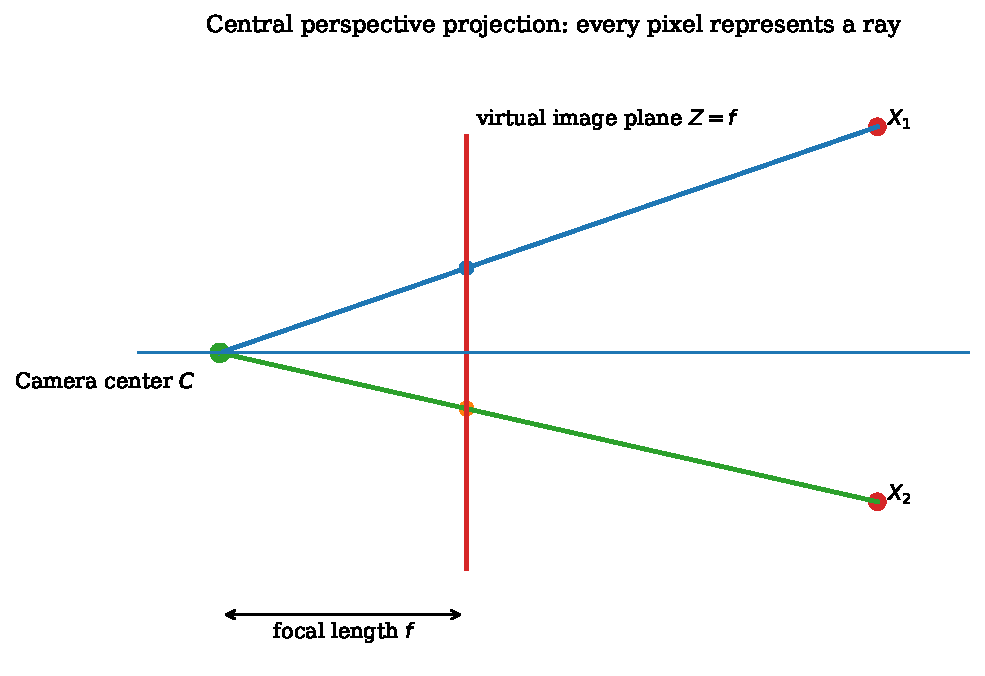
\includegraphics[width=0.88\textwidth]{pinhole_projection.pdf}
\caption{مدل مرکزی دوربین. دو نقطه سه‌بعدی می‌توانند روی یک پرتو قرار گیرند و به یک پیکسل نگاشت شوند؛ ازاین‌رو تصویر تک‌دید به‌تنهایی عمق متریک را تعیین نمی‌کند.}
\label{fig:pinhole}
\end{figure}

مدل دوربین را می‌توان ترکیب چهار نگاشت دانست:
\begin{equation}
\vect X_w
\xrightarrow{\text{وضعیت}}
\vect X_c
\xrightarrow{\text{فرافکنی}}
\vect x_n
\xrightarrow{\text{لنز}}
\vect x_d
\xrightarrow{\text{نمونه‌برداری}}
\vect u.
\label{eq:camera-composition}
\end{equation}
این تجزیه در مهندسی بسیار مهم است؛ زیرا نشان می‌دهد خطا ممکن است از وضعیت، مدل لنز، قرارداد پیکسل یا زمان نوردهی ناشی شود.

\begin{figure}[H]
\centering
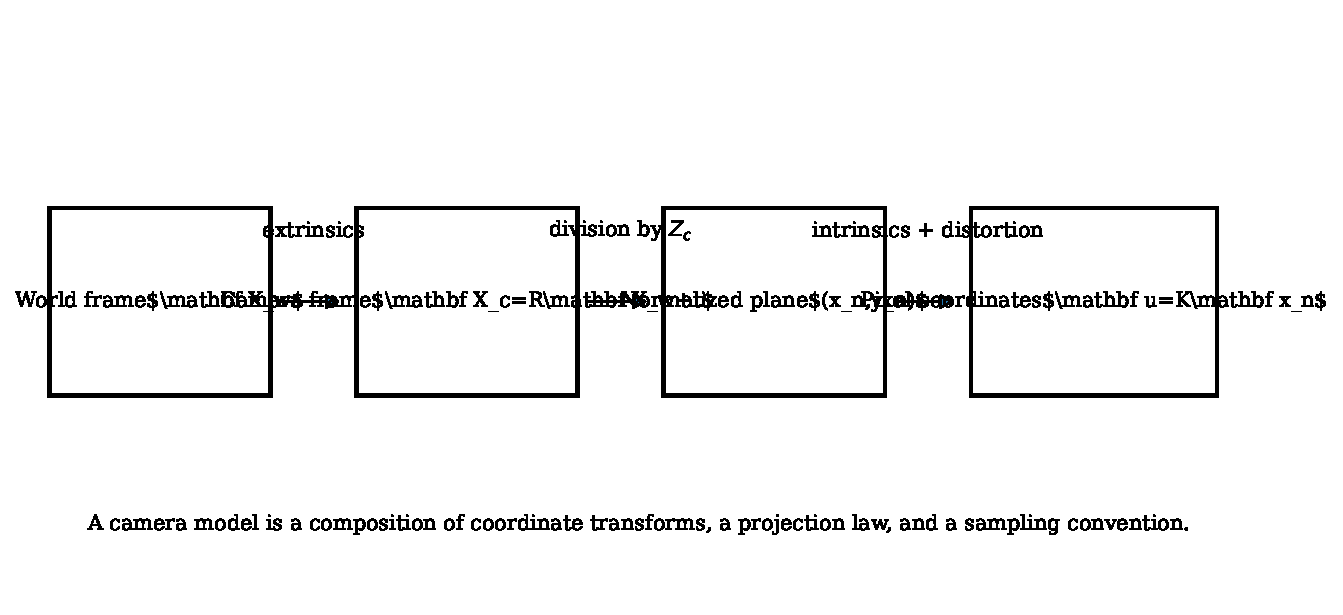
\includegraphics[width=0.95\textwidth]{coordinate_pipeline.pdf}
\caption{زنجیره مختصات در مدل دوربین. دوربین تنها یک ماتریس نیست؛ ترکیب دستگاه مختصات، قانون فرافکنی، اعوجاج و نمونه‌برداری است.}
\label{fig:coordinate-pipeline}
\end{figure}

% =============================================================================
\section{هندسه تصویری و مختصات همگن}
% =============================================================================

\subsection{چرا همگن‌سازی؟}
در صفحه اقلیدسی، انتقال یک تبدیل خطی نیست؛ اما با افزودن یک مؤلفه مقیاس، تمام تبدیلات تصویری به ضرب ماتریسی تبدیل می‌شوند.
نقطه اقلیدسی \((x,y)\) با کلاس هم‌ارزی
\begin{equation}
\widetilde{\vect x}=\lambda(x,y,1)\trans,\qquad \lambda\neq0
\end{equation}
نمایش داده می‌شود. دو بردار همگن که تنها در مقیاس تفاوت دارند یک نقطه از فضای تصویری \(\Pj^2\) را نشان می‌دهند.

خط دوبعدی نیز برداری همگن است:
\begin{equation}
\vect \ell=(a,b,c)\trans,\qquad \vect\ell\trans\widetilde{\vect x}=0.
\end{equation}
تقاطع دو خط و خط گذرنده از دو نقطه با ضرب برداری به‌دست می‌آید:
\begin{equation}
\widetilde{\vect x}=\vect\ell_1\times\vect\ell_2,
\qquad
\vect\ell=\widetilde{\vect x}_1\times\widetilde{\vect x}_2.
\label{eq:incidence-cross}
\end{equation}

\begin{definition}[نقطه بی‌نهایت]
نقطه همگن \((x,y,0)\trans\) یک جهت در صفحه است. خطوط موازی اقلیدسی در فضای تصویری در یک نقطه بی‌نهایت تقاطع دارند.
مجموع نقاط بی‌نهایت خط \(\ell_\infty=(0,0,1)\trans\) را تشکیل می‌دهد.
\end{definition}

این تعریف پایه ریاضی نقطه گریز است: دسته‌ای از خطوط موازی سه‌بعدی پس از فرافکنی در تصویری متناهی یا نقطه‌ای در بی‌نهایت
به هم می‌رسند.

\subsection{تبدیلات دوبعدی و سلسله‌مراتب هندسی}
تبدیل تصویری عمومی یا هموگرافی با ماتریس ناصفر \(\mat H\in\R^{3\times3}\) تعریف می‌شود:
\begin{equation}
\widetilde{\vect x}'\sim\mat H\widetilde{\vect x},\qquad \det(\mat H)\neq0.
\end{equation}
چون مقیاس ماتریس اهمیتی ندارد، هموگرافی هشت درجه آزادی دارد و عضو گروه \(\PGL(3)\) است.

\begin{table}[H]
\centering
\caption{سلسله‌مراتب تبدیلات دوبعدی و کمیت‌های حفظ‌شونده}
\begin{tabularx}{\textwidth}{>{\bfseries}p{2.8cm}p{3.0cm}p{2.6cm}X}
\toprule
تبدیل & شکل ماتریس & درجه آزادی & کمیت‌های حفظ‌شونده\\
\midrule
اقلیدسی & چرخش + انتقال & 3 & فاصله، زاویه، نسبت طول\\
تشابه & مقیاس یکنواخت + اقلیدسی & 4 & زاویه و نسبت طول\\
آفین & بلوک خطی دلخواه + انتقال & 6 & موازی‌بودن، نسبت روی یک خط\\
تصویری & ماتریس همگن دلخواه & 8 & هم‌خطی، تقاطع و نسبت دوگانه\\
\bottomrule
\end{tabularx}
\end{table}

\begin{proposition}[انتقال خط تحت هموگرافی]
اگر نقاط با \(\vect x'\sim H\vect x\) تبدیل شوند، خط‌ها با
\begin{equation}
\vect\ell'\sim H^{-\mathsf T}\vect\ell
\end{equation}
تبدیل می‌شوند.
\end{proposition}
\begin{proof}
از قید برخورد \(\ell\trans x=0\) و \(x\sim H^{-1}x'\) داریم
\(\ell\trans H^{-1}x'=0\)، پس \((H^{-\mathsf T}\ell)\trans x'=0\).
\end{proof}

\subsection{صفحه و خط در فضای سه‌بعدی}
نقطه سه‌بعدی همگن \(\widetilde X\in\Pj^3\) چهار مؤلفه دارد. صفحه
\(\vect\pi=(\vect n\trans,d)\trans\) با قید
\begin{equation}
\vect\pi\trans\widetilde{\vect X}=\vect n\trans\vect X+d=0
\end{equation}
تعریف می‌شود. خط سه‌بعدی به‌سادگی یک بردار چهاربعدی نیست؛ می‌توان آن را با تقاطع دو صفحه یا اتصال دو نقطه نمایش داد.
برای محاسبات چنددیدگاهی، مختصات پلوکر نمایش مناسبی برای خط سه‌بعدی است.

\begin{futurebox}
در مدل‌های «هر دوربینی»، یک پیکسل الزاماً با ماتریس \(K^{-1}\) به پرتو تبدیل نمی‌شود. نمایش عمومی‌تر، نگاشتی از پیکسل به
یک خط سه‌بعدی یا یک جفت مبدأ-جهت است. این دیدگاه برای دوربین‌های غیرمرکزی، آرایه‌های چنددوربینه و رندر عصبی چندحسگری ضروری است.
\end{futurebox}

% =============================================================================
\section{حرکت صلب، چرخش و وضعیت دوربین}
% =============================================================================

\subsection{گروه چرخش سه‌بعدی}
ماتریس چرخش صحیح مجموعه
\begin{equation}
\SO(3)=\{R\in\R^{3\times3}:R\trans R=I,\ \det R=1\}
\end{equation}
است. قید تعامد شش معادله مستقل ایجاد می‌کند؛ بنابراین چرخش سه درجه آزادی دارد.

\begin{warningbox}
پارامترهای اویلر شهودی‌اند، اما ترتیب چرخش اهمیت دارد و در برخی وضعیت‌ها به قفل گیمبال می‌رسند. ماتریس چرخش افزونگی دارد،
کواترنیون قید نرم واحد دارد و محور-زاویه برای بهینه‌سازی محلی مناسب است. هیچ نمایش واحدی برای همه کاربردها بهترین نیست.
\end{warningbox}

برای بردار \(\vect\omega\in\R^3\)، ماتریس پادمتقارن
\begin{equation}
\skewm{\vect\omega}=\begin{bmatrix}
0&-\omega_3&\omega_2\\
\omega_3&0&-\omega_1\\
-\omega_2&\omega_1&0
\end{bmatrix}
\end{equation}
خاصیت \(\skewm{\omega}v=\omega\times v\) دارد. نگاشت نمایی رودریگز چرخش را می‌دهد:
\begin{equation}
R=\Exp(\skewm{\omega})
=I+\frac{\sin\theta}{\theta}\skewm{\omega}
+\frac{1-\cos\theta}{\theta^2}\skewm{\omega}^2,
\qquad \theta=\norm{\omega}.
\label{eq:rodrigues}
\end{equation}

\subsection{گروه حرکت صلب و جبر لی}
وضعیت دوربین در \(\SE(3)\) به‌صورت
\begin{equation}
T=\begin{bmatrix}R&t\\0\trans&1\end{bmatrix}
\end{equation}
نوشته می‌شود. برای بهینه‌سازی، تغییر کوچک شش‌بعدی
\(\vect\xi=(\vect\rho\trans,\vect\omega\trans)\trans\)
در جبر لی \(\mathfrak{se}(3)\) تعریف و با
\begin{equation}
T\leftarrow\Exp(\vect\xi^\wedge)T
\end{equation}
اعمال می‌شود. مزیت این کار آن است که تکرار بهینه‌سازی روی فضای مینیمال انجام می‌شود و ماتریس چرخش از گروه خارج نمی‌شود.

\begin{proofbox}[ژاکوبین فرافکنی نسبت به وضعیت]
برای نقطه دوربینی \(X_c=(X,Y,Z)\trans\) و مختصات نرمال
\(x=X/Z,\ y=Y/Z\)، ژاکوبین فرافکنی نسبت به نقطه برابر است با
\begin{equation}
J_\pi=\begin{bmatrix}
1/Z&0&-X/Z^2\\
0&1/Z&-Y/Z^2
\end{bmatrix}.
\end{equation}
اگر اغتشاش چپ‌ضرب باشد، تغییر نقطه دوربینی
\(\delta X_c\simeq \rho-\skewm{X_c}\omega\) است؛ پس
\begin{equation}
J_{\pi,\xi}=J_\pi\begin{bmatrix}I&-\skewm{X_c}\end{bmatrix}.
\end{equation}
این ژاکوبین هسته محاسبات \lr{visual odometry}، \lr{bundle adjustment} و رندر تفاضل‌پذیر است.
\end{proofbox}

% =============================================================================
\section{استخراج دوربین سوراخ‌سوزنی}
% =============================================================================

\subsection{فرافکنی نرمال}
در دستگاه دوربین، نقطه \(X_c=(X_c,Y_c,Z_c)\trans\) با \(Z_c>0\) به صفحه نرمال نگاشت می‌شود:
\begin{equation}
\vect x_n=\pi(\vect X_c)=
\begin{bmatrix}X_c/Z_c\\Y_c/Z_c\end{bmatrix}.
\label{eq:normalized-projection}
\end{equation}
به‌شکل همگن:
\begin{equation}
\widetilde{\vect x}_n\sim
\begin{bmatrix}I_{3\times3}&0\end{bmatrix}
\widetilde{\vect X}_c.
\end{equation}

\subsection{ماتریس پارامترهای درونی}
تبدیل مختصات نرمال به پیکسل با
\begin{equation}
K=\begin{bmatrix}
f_x&s&c_x\\
0&f_y&c_y\\
0&0&1
\end{bmatrix}
\label{eq:intrinsic}
\end{equation}
انجام می‌شود. در این رابطه \(f_x=f/p_x\) و \(f_y=f/p_y\) فاصله کانونی بر حسب پیکسل،
\((c_x,c_y)\) نقطه اصلی و \(s\) کجی محورهای پیکسلی است.

ترکیب وضعیت و درونی‌ها می‌دهد:
\begin{equation}
\widetilde{\vect u}\sim
K\begin{bmatrix}R&t\end{bmatrix}\widetilde{\vect X}_w
=P\widetilde{\vect X}_w.
\label{eq:camera-matrix}
\end{equation}
ماتریس \(P\in\R^{3\times4}\) یازده درجه آزادی دارد، اما دوربین متریک با ساختار \(K[R|t]\) محدودتر است.

\begin{figure}[H]
\centering
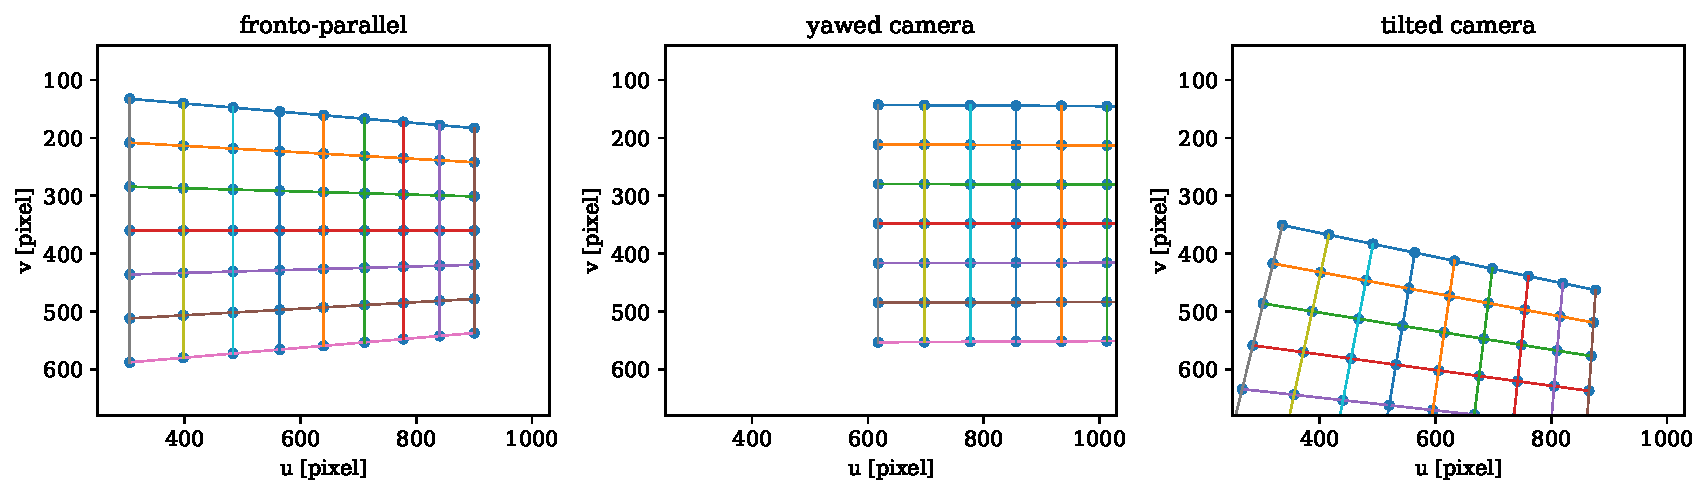
\includegraphics[width=0.98\textwidth]{perspective_foreshortening.pdf}
\caption{فشردگی پرسپکتیو برای یک شبکه سه‌بعدی. تغییر وضعیت دوربین، خطوط و فاصله‌های تصویری را به‌صورت غیرخطی تغییر می‌دهد، هرچند نگاشت همگن خطی است.}
\label{fig:foreshortening}
\end{figure}

\subsection{مرکز دوربین و تجزیه ماتریس دوربین}
مرکز دوربین بردار ناصفر فضای تهی راست \(P\) است:
\begin{equation}
P\widetilde C=0.
\end{equation}
اگر \(P=[M\mid p_4]\) و \(M\) وارون‌پذیر باشد،
\begin{equation}
\widetilde C\sim\begin{bmatrix}-M^{-1}p_4\\1\end{bmatrix}.
\end{equation}
برای استخراج \(K\) و \(R\) از \(M\)، تجزیه \lr{RQ} به‌کار می‌رود؛ علامت قطر \(K\) و دترمینان \(R\) باید اصلاح شود.

\subsection{میدان دید و ارتباط واحد فیزیکی و پیکسلی}
اگر عرض حسگر \(W_s\) و فاصله کانونی فیزیکی \(f\) باشد، میدان دید افقی تقریباً
\begin{equation}
\mathrm{FOV}_x=2\arctan\frac{W_s}{2f}
\end{equation}
است. برش دیجیتال، تغییر اندازه و \lr{binning} می‌توانند \(f_x,c_x\) را تغییر دهند بدون آنکه لنز فیزیکی عوض شود.

\begin{example}[تغییر پارامتر درونی تحت تغییر اندازه]
اگر تصویر با ضرایب \(s_x,s_y\) تغییر اندازه یابد،
\begin{equation}
K'=\begin{bmatrix}s_x&0&0\\0&s_y&0\\0&0&1\end{bmatrix}K.
\end{equation}
بنابراین استفاده از ماتریس کالیبراسیون یک رزولوشن برای رزولوشن دیگر، بدون مقیاس‌دهی، نادرست است.
\end{example}

% =============================================================================
\section{لنز نازک، فوکوس و هندسه نوردهی}
% =============================================================================

مدل سوراخ‌سوزنی عمق میدان نامتناهی و نور ناچیز دارد. لنز نازک توان جمع‌آوری نور را افزایش می‌دهد و رابطه
\begin{equation}
\frac{1}{f}=\frac{1}{z_o}+\frac{1}{z_i}
\label{eq:thin-lens}
\end{equation}
میان فاصله شیء \(z_o\)، فاصله تصویر \(z_i\) و فاصله کانونی برقرار می‌کند. اگر حسگر دقیقاً روی صفحه تصویر متناظر نباشد،
نقطه به دیسکی با شعاع «دایره اغتشاش» تبدیل می‌شود.

برای قطر دهانه \(A=f/N\) با عدد \(f\)-استاپ \(N\)، قطر تقریبی دایره اغتشاش برای شیئی در عمق \(z\) و فوکوس روی \(z_f\) از هندسه مشابهت مثلث‌ها به‌دست می‌آید. این بحث نشان می‌دهد تاری خارج از فوکوس
\textbf{عمق‌وابسته} است و عموماً با یک کانولوشن ناوردا مدل نمی‌شود.

\begin{futurebox}
دوربین‌های محاسباتی آینده، وضعیت، عمق، دیافراگم و حتی حرکت حسگر را هم‌زمان بهینه می‌کنند. از دید ریاضی، مرز میان
«کالیبراسیون» و «بازسازی» محو می‌شود: پارامترهای اپتیکی و صحنه در یک مسئله معکوس مشترک تخمین زده می‌شوند.
\end{futurebox}

% =============================================================================
\section{اعوجاج لنز و مدل‌های دوربین عریض}
% =============================================================================

\subsection{مدل براون-کنرادی}
برای مختصات نرمال ایده‌آل \((x,y)\)، \(r^2=x^2+y^2\). مدل شعاعی-مماسی رایج می‌نویسد:
\begin{align}
x_d&=x(1+k_1r^2+k_2r^4+k_3r^6)
+2p_1xy+p_2(r^2+2x^2),\\
y_d&=y(1+k_1r^2+k_2r^4+k_3r^6)
+p_1(r^2+2y^2)+2p_2xy.
\label{eq:brown}
\end{align}
پارامترهای \(k_i\) اعوجاج شعاعی و \(p_i\) نامرکزبودن اجزای لنز را مدل می‌کنند. مدل‌های عقلانی، منشور نازک و کجی حسگر
برای لنزهای دشوارتر پارامترهای بیشتری می‌افزایند.

\begin{figure}[H]
\centering
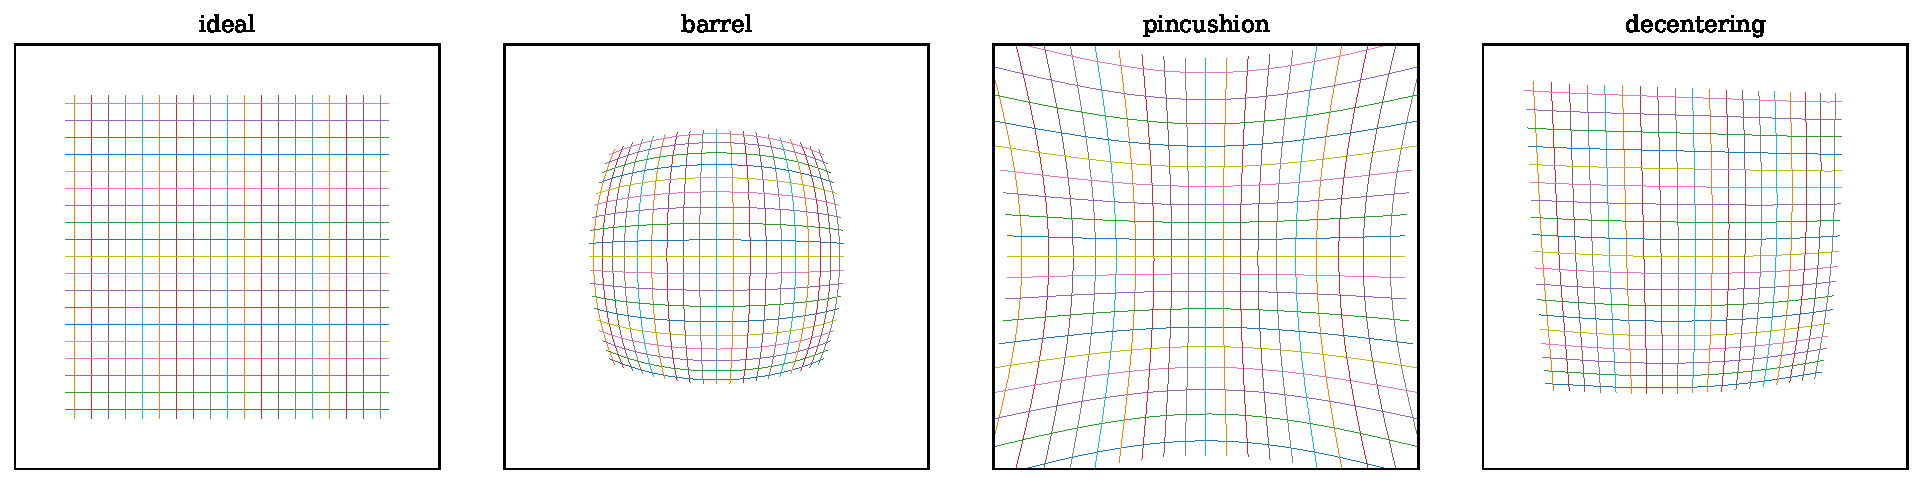
\includegraphics[width=0.98\textwidth]{distortion_models.pdf}
\caption{اثر کیفی مدل‌های اعوجاج بر شبکه مستقیم. اعوجاج باید در مختصات نرمال و با قرارداد دقیق مدل نرم‌افزار اعمال شود.}
\label{fig:distortion}
\end{figure}

\begin{warningbox}
افزودن ضرایب بیشتر همیشه کالیبراسیون را بهتر نمی‌کند. مدل پرپارامتر می‌تواند خطای بازفرافکنی آموزش را کاهش دهد، اما در
حاشیه تصویر یا فاصله‌های فوکوس دیگر ناپایدار شود. انتخاب مدل باید با اعتبارسنجی خارج از داده برازش، نمودار باقیمانده و
شرطی‌بودن ژاکوبین انجام گیرد.
\end{warningbox}

\subsection{قوانین فرافکنی چشم‌ماهی}
در دوربین عریض، زاویه فرودی \(\theta\) به شعاع تصویری \(r\) با قوانین مختلف نگاشت می‌شود:
\begin{align}
\text{پرسپکتیو: }&r=f\tan\theta,\\
\text{هم‌فاصله: }&r=f\theta,\\
\text{هم‌جامد: }&r=2f\sin(\theta/2),\\
\text{استریوگرافیک: }&r=2f\tan(\theta/2),\\
\text{متعامد: }&r=f\sin\theta.
\end{align}
مدل کانالا-برنت زاویه را با چندجمله‌ای فرد پارامتری می‌کند:
\begin{equation}
\theta_d=\theta(1+k_1\theta^2+k_2\theta^4+k_3\theta^6+k_4\theta^8),
\qquad
(x_d,y_d)=\frac{\theta_d}{r}(x,y).
\label{eq:kb}
\end{equation}

\begin{figure}[H]
\centering
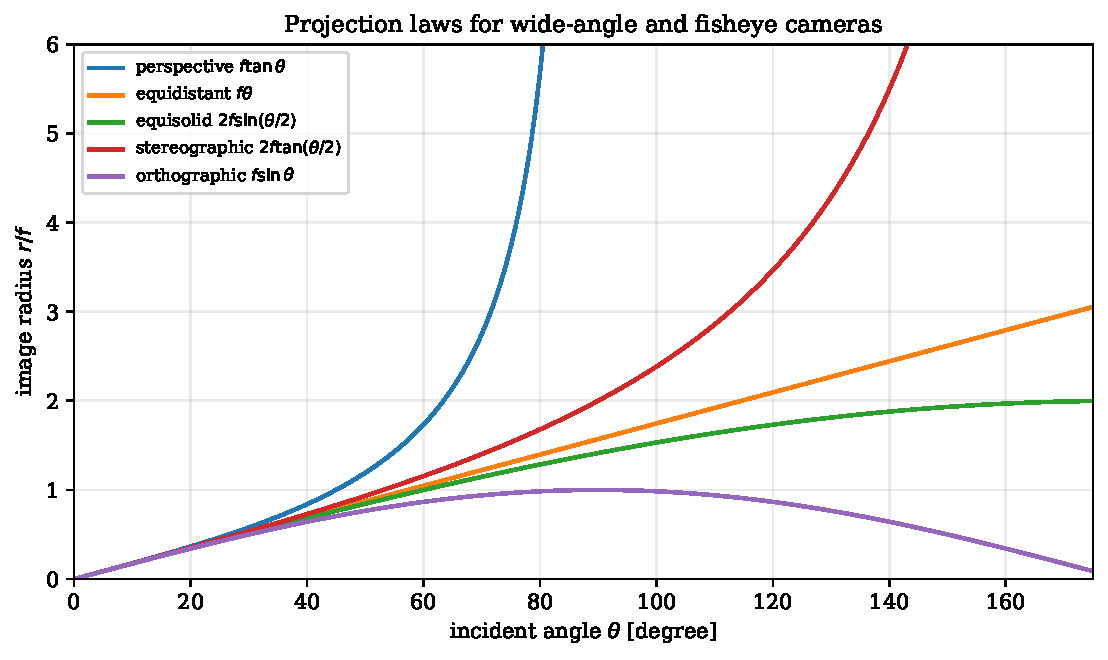
\includegraphics[width=0.78\textwidth]{fisheye_projection_laws.pdf}
\caption{مقایسه قوانین فرافکنی زاویه به شعاع. مدل پرسپکتیو در نزدیک ۹۰ درجه واگرا می‌شود؛ دوربین چشم‌ماهی با قانون دیگری میدان دید بسیار بزرگ را پوشش می‌دهد.}
\label{fig:fisheye-laws}
\end{figure}

\subsection{مدل یکپارچه همه‌جهته و دوربین غیرمرکزی}
در دوربین کاتادیوپتریک مرکزی، پرتو ابتدا روی کره واحد نگاشت و سپس از یک مرکز مجازی به صفحه تصویر فرافکنی می‌شود.
پارامتر \(\xi\) فاصله مرکز کره تا مرکز فرافکنی را کنترل می‌کند. این مدل، دوربین پرسپکتیو و برخی سامانه‌های آینه‌ای را در
یک خانواده قرار می‌دهد.

دوربین غیرمرکزی یک مرکز مشترک برای همه پرتوها ندارد. دوربین چندکانونی، آرایه دوربین، سامانه \lr{push-broom} و برخی
لنزهای بسیار عریض به نمایش عمومی‌تر نیاز دارند:
\begin{equation}
\vect u\longmapsto (\vect o(\vect u),\vect d(\vect u)),
\end{equation}
که در آن هر پیکسل مبدأ و جهت پرتو مخصوص خود را دارد.

\begin{researchbox}[مدل مناسب را بر اساس داده انتخاب کنید]
در نرم‌افزارهای بازسازی جدید، مدل‌های ساده شعاعی برای تصاویر اینترنتی با درونی‌های نامعلوم، مدل \lr{OpenCV} برای دوربین
معمولی کالیبره، مدل کانالا-برنت برای چشم‌ماهی و مدل‌های همه‌جهته برای آینه-لنز استفاده می‌شوند. معیار اصلی کمترین تعداد
پارامتری است که ساختار سیستماتیک باقیمانده را حذف کند، نه کمترین خطای آموزش به هر قیمت.
\end{researchbox}

% =============================================================================
\section{هندسه تک‌دید: نقطه گریز، خط افق و هموگرافی}
% =============================================================================

\subsection{نقطه گریز جهت سه‌بعدی}
برای جهت جهان \(\vect d\) و دوربین \(P=K[R|t]\)، نقطه بی‌نهایت \((\vect d\trans,0)\trans\) به
\begin{equation}
\vect v\sim KR\vect d
\label{eq:vanishing}
\end{equation}
نگاشت می‌شود. انتقال دوربین در نقطه گریز ظاهر نمی‌شود؛ بنابراین نقاط گریز اطلاعاتی درباره جهت‌گیری، نه مکان دوربین، می‌دهند.

اگر دو جهت جهان متعامد باشند، با \(\omega=K^{-\mathsf T}K^{-1}\) داریم
\begin{equation}
\vect v_i\trans\omega\vect v_j=0.
\end{equation}
این قید مبنای کالیبراسیون از صحنه منهتن و تصویر مخروط مطلق است.

\subsection{هموگرافی صفحه}
برای صفحه جهان \(\pi:n\trans X+d=0\)، نگاشت میان دو تصویر یک هموگرافی است. اگر دوربین‌ها
\(P_1=K_1[I|0]\) و \(P_2=K_2[R|t]\) باشند:
\begin{equation}
H_{21}=K_2\left(R-\frac{tn\trans}{d}\right)K_1^{-1}.
\label{eq:plane-homography}
\end{equation}
در چرخش خالص یا صحنه کاملاً تخت، همه نقاط با یک هموگرافی مرتبط‌اند؛ در صحنه عمومی با ترجمه، یک هموگرافی واحد کافی نیست.

\subsection{تصحیح تصویری و اندازه‌گیری تک‌دید}
با تخمین تصویر خط بی‌نهایت می‌توان اعوجاج تصویری یک صفحه را تا هندسه آفین حذف کرد. با افزودن قیود تعامد یا طول،
تصحیح متریک ممکن می‌شود. نسبت دوگانه چهار نقطه هم‌خط تحت هموگرافی ثابت است:
\begin{equation}
(A,B;C,D)=\frac{AC/BC}{AD/BD}.
\end{equation}
این ناوردایی مبنای اندازه‌گیری ارتفاع و فاصله از یک تصویر با اطلاعات مرجع است.

% =============================================================================
\section{برآورد ماتریس دوربین با DLT}
% =============================================================================

برای هر تطابق \(\widetilde X_i\leftrightarrow\widetilde u_i\)، قید
\(\widetilde u_i\times P\widetilde X_i=0\) سه معادله می‌دهد که دو معادله مستقل‌اند. با چیدن ضرایب:
\begin{equation}
A\vect p=0,
\end{equation}
که \(\vect p\) بردارسازی \(P\) است. پاسخ کمترین مربعات همگن، بردار منفرد راست متناظر با کوچک‌ترین مقدار منفرد \(A\) است.

\begin{proofbox}[چرا نرمال‌سازی ضروری است؟]
مختصات پیکسلی ممکن است در مرتبه هزار و مختصات همگن ثابت در مرتبه یک باشند. این اختلاف مقیاس، دستگاه \(A\) را بدشرط
می‌کند. تبدیل تشابهی که مرکز نقاط را صفر و فاصله متوسط را \(\sqrt{2}\) در دوبعد و \(\sqrt{3}\) در سه‌بعد می‌کند،
شرطی‌بودن را بهبود می‌دهد. پس از تخمین باید تبدیل‌ها بازگردانده شوند.
\end{proofbox}

\begin{warningbox}
\lr{DLT} یک مقداردهی اولیه جبری است، نه پاسخ نهایی آماری. خطای جبری \(\norm{Ap}\) با خطای پیکسلی یکسان نیست و
ناهمسانی و برون‌زدگی را به‌درستی مدل نمی‌کند. پاسخ نهایی باید خطای بازفرافکنی را با مدل نویز مناسب کمینه کند.
\end{warningbox}

% =============================================================================
\section{کالیبراسیون دوربین: از صفحه ژانگ تا پالایش غیرخطی}
% =============================================================================

\subsection{صورت‌بندی کالیبراسیون}
داده کالیبراسیون مجموعه نقاط معلوم \(X_{ij}\) و مشاهدات پیکسلی \(u_{ij}\) در نماهای متعدد است. مجهولات شامل
پارامترهای درونی \(\theta_K\)، اعوجاج \(\theta_d\) و وضعیت هر نما \((R_i,t_i)\) است:
\begin{equation}
\min_{\theta_K,\theta_d,\{R_i,t_i\}}
\sum_i\sum_j
\rho\!\left(
\norm{u_{ij}-\Pi(X_{ij};\theta_K,\theta_d,R_i,t_i)}_{\Sigma_{ij}^{-1}}^2
\right).
\label{eq:calib-objective}
\end{equation}

\subsection{استخراج بسته روش ژانگ}
صفحه کالیبراسیون را \(Z=0\) می‌گیریم. برای نمای \(i\):
\begin{equation}
\widetilde u\sim K\begin{bmatrix}r_1&r_2&t\end{bmatrix}
\begin{bmatrix}X\\Y\\1\end{bmatrix}
=H_i\widetilde X_\pi.
\end{equation}
اگر ستون‌های هموگرافی \(H=[h_1,h_2,h_3]\) باشند، تا ضریب \(\lambda\):
\begin{equation}
h_1=\lambda Kr_1,\qquad h_2=\lambda Kr_2.
\end{equation}
از تعامد و برابری نرم \(r_1,r_2\):
\begin{align}
h_1\trans B h_2&=0,\\
h_1\trans B h_1-h_2\trans B h_2&=0,
\label{eq:zhang-constraints}
\end{align}
که
\begin{equation}
B=K^{-\mathsf T}K^{-1}
\end{equation}
ماتریسی متقارن با شش مؤلفه و مقیاس نامعین است. هر نما دو قید خطی می‌دهد. با حداقل سه نمای مناسب، \(B\) و سپس \(K\)
استخراج می‌شود. وضعیت هر نما از \(K^{-1}H\) و متعامدسازی به‌دست می‌آید؛ سپس همه پارامترها با مسئله
\eqref{eq:calib-objective} پالایش می‌شوند.

\begin{figure}[H]
\centering
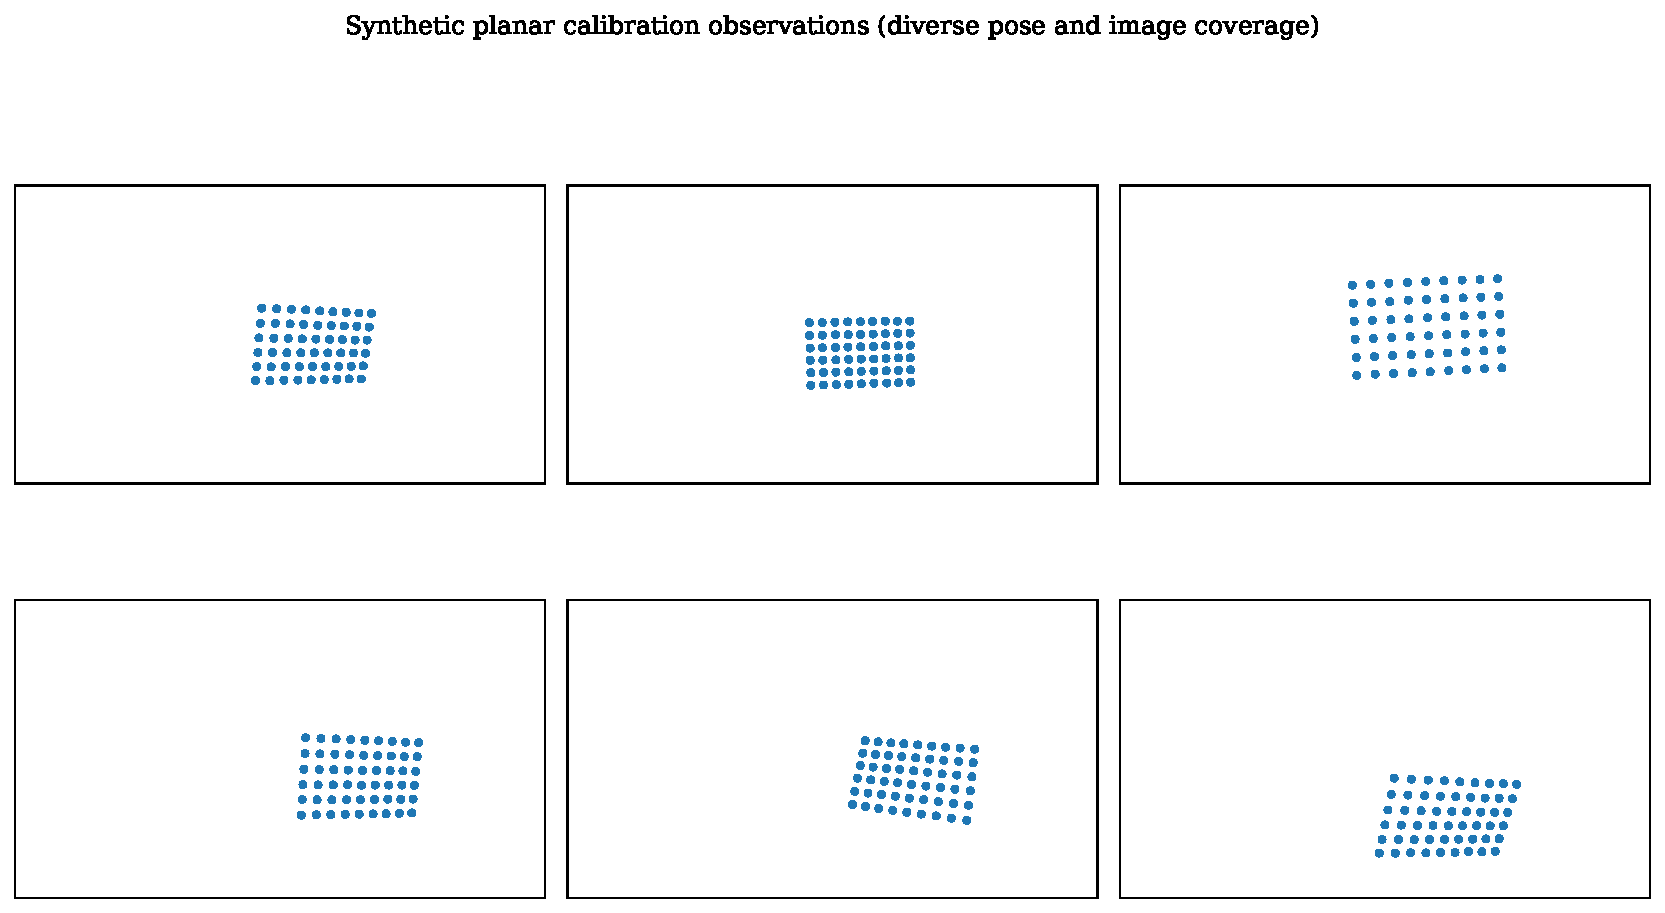
\includegraphics[width=0.9\textwidth]{calibration_views.pdf}
\caption{چند نمای مصنوعی از صفحه کالیبراسیون. تنوع زاویه، عمق و پوشش حاشیه تصویر برای مشاهده‌پذیری پارامترهای درونی و اعوجاج ضروری است.}
\label{fig:calib-views}
\end{figure}

\subsection{شرایط تباه و طراحی داده}
موارد زیر کالیبراسیون را ضعیف می‌کنند:
\begin{itemize}
\item همه نماها تقریباً روبه‌رو و در یک فاصله باشند؛
\item هدف تنها مرکز تصویر را بپوشاند و حاشیه‌ها دیده نشوند؛
\item فوکوس، زوم یا رزولوشن میان نماها تغییر کند ولی یک \(K\) مشترک فرض شود؛
\item صفحه کالیبراسیون تاب‌دار، چاپ مقیاس‌خورده یا نقاط گوشه با خطای سیستماتیک باشد؛
\item مدل اعوجاج بسیار ساده یا بیش‌ازحد پرپارامتر باشد.
\end{itemize}

\begin{figure}[H]
\centering
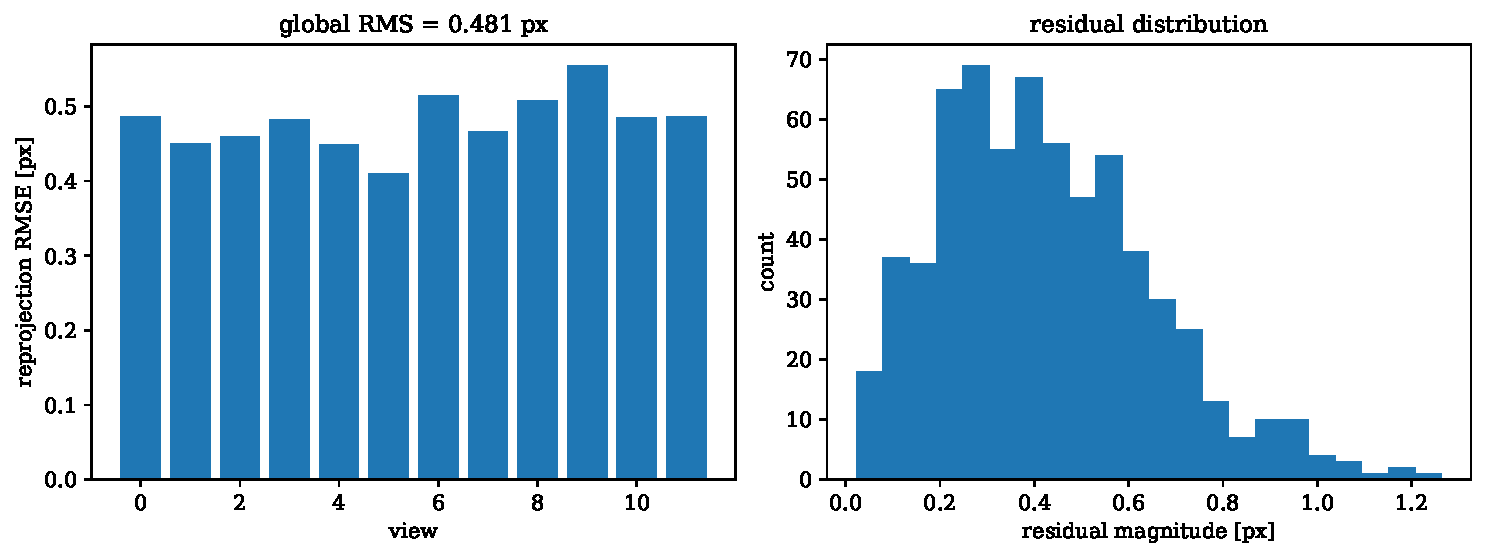
\includegraphics[width=0.82\textwidth]{calibration_residuals.pdf}
\caption{خطای بازفرافکنی آزمایش مصنوعی فصل. علاوه بر میانگین کلی باید خطای هر نما و توزیع باقیمانده بررسی شود.}
\label{fig:calib-residuals}
\end{figure}

\subsection{عدم‌قطعیت کالیبراسیون}
در نزدیکی پاسخ، باقیمانده \(r(\theta)\) خطی می‌شود:
\begin{equation}
r(\theta+\delta)\simeq r(\theta)+J\delta.
\end{equation}
برای نویز گاوسی با کوواریانس \(\Sigma\)، تقریب کوواریانس پارامترها
\begin{equation}
\Cov(\widehat\theta)\simeq(J\trans\Sigma^{-1}J)^{-1}
\label{eq:calib-cov}
\end{equation}
است. مقادیر ویژه کوچک ماتریس اطلاعات، جهت‌های ضعیف مشاهده‌شده را نشان می‌دهند.

\begin{keybox}[خطای بازفرافکنی کم کافی نیست]
یک مدل می‌تواند با پارامترهای غیرواقعی خطای پیکسلی کم داشته باشد، مخصوصاً اگر داده محدود یا مدل پرپارامتر باشد.
اعتبارسنجی باید شامل پایداری پارامتر بین زیرمجموعه‌ها، خطای حاشیه تصویر، بازسازی سه‌بعدی روی فاصله معلوم، نمودار برداری
باقیمانده و حساسیت به حذف هر نما باشد.
\end{keybox}

\begin{workshopbox}[آزمایش مصنوعی کالیبراسیون]
اسکریپت همراه، صفحه \(9\times6\) را در چند وضعیت تصادفی فرافکنی می‌کند، اعوجاج و نویز زیرپیکسلی می‌افزاید و با
\texttt{cv2.calibrateCamera} پارامترها را تخمین می‌زند. فایل‌های
\texttt{calibration\_summary.csv} و \texttt{calibration\_per\_view.csv}
برای تحلیل خطا ذخیره می‌شوند. دانشجو باید آزمایش را برای تعداد نما، دامنه زاویه، شدت اعوجاج و نویز گوشه تکرار کند.
\end{workshopbox}

% =============================================================================
\section{هندسه دو دید و قید اپی‌پولار}
% =============================================================================

\subsection{صفحه اپی‌پولار}
دو مرکز دوربین \(C_1,C_2\) و نقطه سه‌بعدی \(X\) صفحه‌ای تشکیل می‌دهند. تقاطع این صفحه با هر صفحه تصویر یک خط
اپی‌پولار است. بنابراین تطابق نقطه در تصویر دوم به جای کل صفحه روی یک خط جست‌وجو می‌شود.

برای دوربین‌های کالیبره با مختصات نرمال \(x_1,x_2\) و حرکت نسبی \((R,t)\):
\begin{equation}
x_2\trans E x_1=0,
\qquad
E=\skewm{t}R.
\label{eq:essential}
\end{equation}
ماتریس اساسی \(E\) رتبه دو و دو مقدار منفرد برابر دارد.

برای مختصات پیکسلی:
\begin{equation}
u_2\trans F u_1=0,
\qquad
F=K_2^{-\mathsf T}EK_1^{-1}.
\label{eq:fundamental}
\end{equation}
ماتریس بنیادی هفت درجه آزادی دارد: نه مؤلفه، منهای مقیاس و قید رتبه دو.

\subsection{الگوریتم هشت‌نقطه‌ای نرمال‌شده}
هر تطابق \((u_i,v_i)\leftrightarrow(u_i',v_i')\) یک معادله خطی در عناصر \(F\) می‌دهد:
\begin{equation}
[u_i'u_i,\ u_i'v_i,\ u_i',\ v_i'u_i,\ v_i'v_i,\ v_i',\ u_i,\ v_i,\ 1]\vect f=0.
\end{equation}
پس از حل \(Af=0\)، باید \(F\) به نزدیک‌ترین ماتریس رتبه دو فرافکنی شود: اگر
\(F=U\diag(\sigma_1,\sigma_2,\sigma_3)V\trans\)، آنگاه
\begin{equation}
\widehat F=U\diag(\sigma_1,\sigma_2,0)V\trans.
\end{equation}
نرمال‌سازی نقاط پیش و بازگردانی تبدیل‌ها پس از حل، برای پایداری ضروری است.

\subsection{فاصله سامپسون}
خطای جبری \(x_2\trans Fx_1\) واحد هندسی ندارد. تقریب مرتبه اول فاصله هندسی دوطرفه، خطای سامپسون است:
\begin{equation}
d_S^2=
\frac{(x_2\trans Fx_1)^2}
{(Fx_1)_1^2+(Fx_1)_2^2+(F\trans x_2)_1^2+(F\trans x_2)_2^2}.
\label{eq:sampson}
\end{equation}

\begin{figure}[H]
\centering
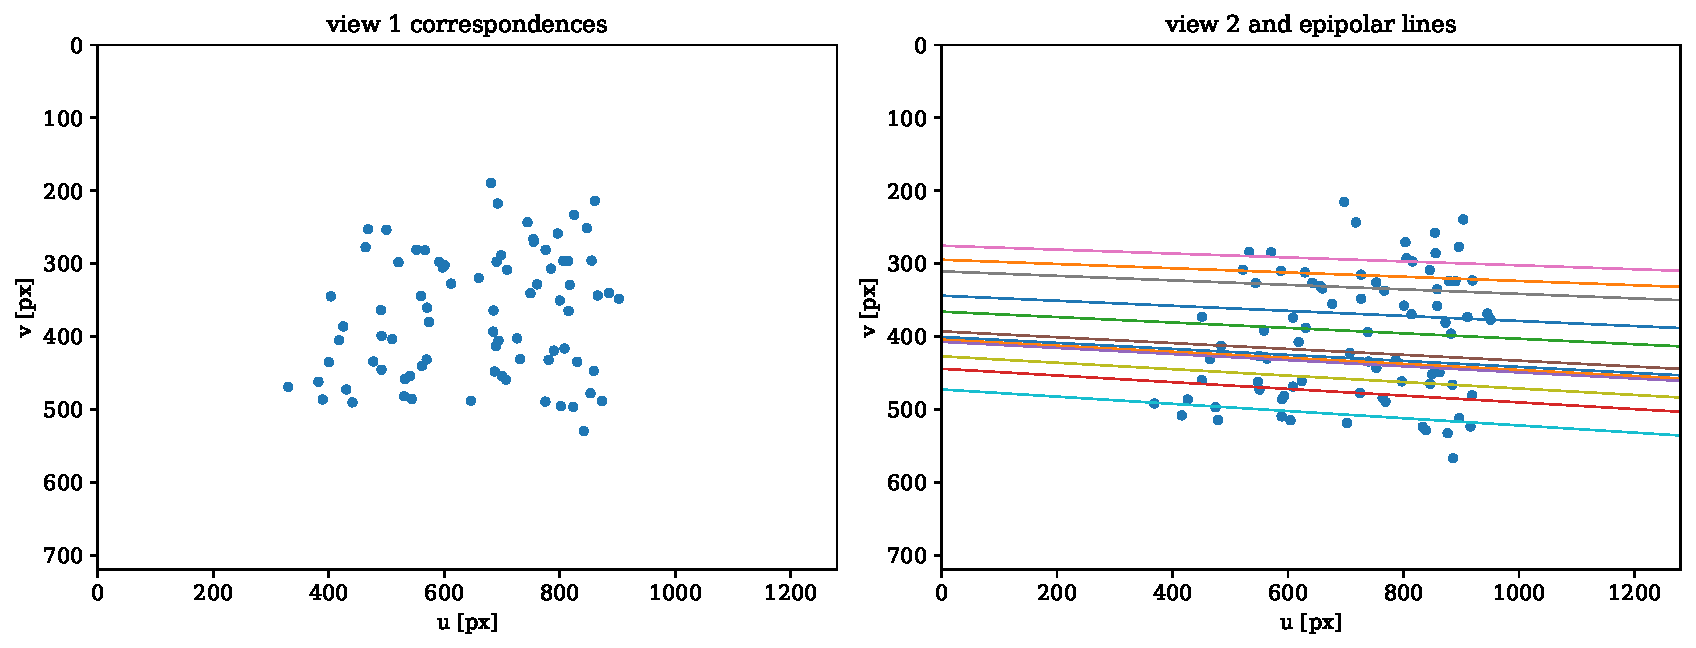
\includegraphics[width=0.9\textwidth]{epipolar_lines.pdf}
\caption{نقاط متناظر مصنوعی و خط‌های اپی‌پولار حاصل از تخمین هشت‌نقطه‌ای. خط باید از همتای نقطه در تصویر دوم عبور کند؛ فاصله باقیمانده معیار کیفیت مدل است.}
\label{fig:epipolar-lines}
\end{figure}

\subsection{تخمین مقاوم و RANSAC}
در حضور تطابق غلط، کمترین مربعات فرو می‌ریزد. \lr{RANSAC} نمونه مینیمال برمی‌گزیند، مدل می‌سازد، درون‌زدها را با آستانه
هندسی می‌شمارد و مدل برتر را با همه درون‌زدها پالایش می‌کند. اگر احتمال درون‌زد \(w\)، اندازه نمونه \(s\) و احتمال موفقیت
\(p\) باشد، تعداد تکرار لازم تقریباً
\begin{equation}
N=\frac{\log(1-p)}{\log(1-w^s)}
\end{equation}
است. آستانه باید بر حسب عدم‌قطعیت پیکسلی و مدل خطا انتخاب شود، نه یک ثابت جادویی.

\begin{warningbox}
حرکت چرخش خالص، صفحه غالب، خط پایه بسیار کوچک و نقاط نزدیک یک صفحه می‌توانند تخمین \(F/E\) و انتخاب میان هموگرافی و
مدل اپی‌پولار را مبهم کنند. سامانه عملی باید تباهی مدل را تشخیص دهد، نه اینکه همواره یک حل‌گر را اجرا کند.
\end{warningbox}

% =============================================================================
\section{بازیابی وضعیت نسبی و مثلث‌بندی}
% =============================================================================

\subsection{تجزیه ماتریس اساسی}
اگر \(E=U\diag(1,1,0)V\trans\)، با
\begin{equation}
W=\begin{bmatrix}0&-1&0\\1&0&0\\0&0&1\end{bmatrix}
\end{equation}
چهار پاسخ نامزد داریم:
\begin{equation}
R=UWV\trans\ \text{یا}\ UW\trans V\trans,
\qquad
 t=\pm u_3.
\end{equation}
قید راست‌دستی اصلاح می‌شود و پاسخ با آزمون \textbf{مثبت‌بودن عمق} یا \lr{cheirality} انتخاب می‌گردد.
مقیاس \(t\) از دو تصویر تک‌چشمی قابل تعیین نیست.

\subsection{مثلث‌بندی خطی}
برای دوربین‌های \(P_i\) و مشاهدات \(x_i\):
\begin{equation}
x_i\times P_iX=0.
\end{equation}
چیدن معادلات دو نما دستگاه \(AX=0\) می‌دهد. راه‌حل خطی نقطه شروع است؛ پاسخ هندسی بهتر، کمینه‌سازی خطای بازفرافکنی است:
\begin{equation}
\widehat X=\argmin_X\sum_i\norm{u_i-\pi(P_iX)}^2.
\end{equation}

\subsection{هندسه عدم‌قطعیت مثلث‌بندی}
وقتی دو پرتو تقریباً موازی‌اند، محل تقاطع بسیار حساس می‌شود. زاویه تقاطع کوچک، خط پایه کوچک، عمق زیاد یا خطای پیکسلی
بزرگ موجب کوواریانس عمق زیاد می‌شود. در طراحی حسگر باید هندسه دید را همانند کیفیت آشکارساز جدی گرفت.

% =============================================================================
\section{استریو، تصحیح و عدم‌قطعیت عمق}
% =============================================================================

برای استریوی تصحیح‌شده با فاصله کانونی \(f\)، خط پایه \(B\) و اختلاف منظر \(d=u_L-u_R\):
\begin{equation}
Z=\frac{fB}{d}.
\label{eq:stereo-depth}
\end{equation}
انتشار خطای مرتبه اول می‌دهد:
\begin{equation}
\sigma_Z\simeq\left|\frac{\partial Z}{\partial d}\right|\sigma_d
=\frac{Z^2}{fB}\sigma_d.
\label{eq:depth-uncertainty}
\end{equation}
بنابراین خطای عمق با مربع فاصله رشد می‌کند.

\begin{figure}[H]
\centering
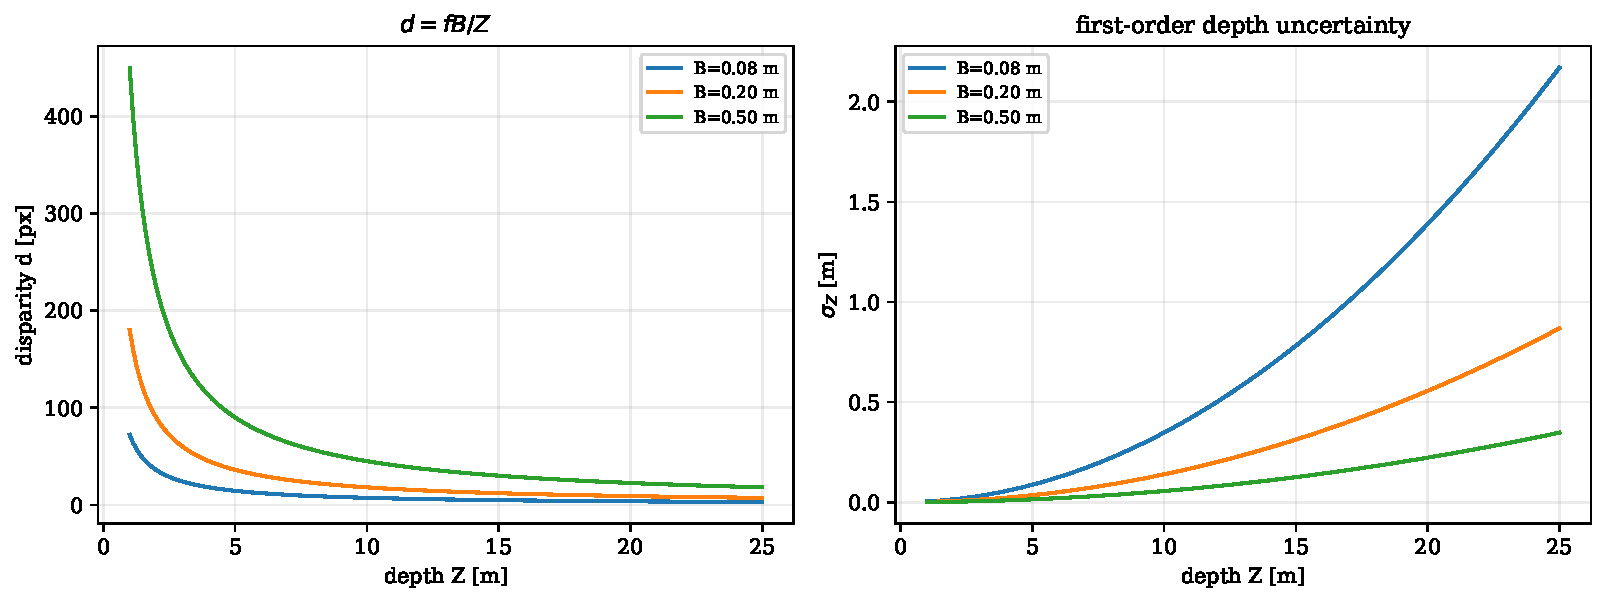
\includegraphics[width=0.88\textwidth]{stereo_depth_uncertainty.pdf}
\caption{رابطه اختلاف منظر و عدم‌قطعیت عمق برای خط پایه‌های مختلف. افزایش خط پایه حساسیت عمق را بهبود می‌دهد، اما همپوشانی دید و پنهان‌شدگی را دشوارتر می‌کند.}
\label{fig:stereo-uncertainty}
\end{figure}

\subsection{تصحیح استریو}
تصحیح، دو تصویر را با هموگرافی‌هایی تبدیل می‌کند تا خطوط اپی‌پولار افقی و متناظر شوند. این کار جست‌وجوی دوبعدی را به
جست‌وجوی یک‌بعدی تبدیل می‌کند. برای دوربین چشم‌ماهی یا همه‌جهته، تصحیح باید با مدل پرتو صحیح انجام شود؛ تبدیل کور به
پرسپکتیو ممکن است حاشیه‌ها را شدیداً کش دهد.

\subsection{انتخاب خط پایه}
خط پایه بزرگ‌تر عمق را دقیق‌تر می‌کند، اما:
\begin{itemize}
\item ناحیه همپوشان کمتر می‌شود؛
\item پنهان‌شدگی و تفاوت ظاهر افزایش می‌یابد؛
\item تطابق برای اجسام نزدیک سخت‌تر می‌شود؛
\item سازه مکانیکی و کالیبراسیون خارجی حساس‌تر می‌شود.
\end{itemize}
پس طراحی استریو یک مسئله چندهدفه است، نه صرفاً بیشینه‌کردن \(B\).

% =============================================================================
\section{وضعیت مطلق: PnP و هندسه ربات-دوربین}
% =============================================================================

مسئله \lr{Perspective-n-Point} از تطابق‌های سه‌بعدی-دوبعدی، وضعیت دوربین را می‌یابد:
\begin{equation}
\min_{R,t}\sum_i\rho\left(\norm{u_i-\pi(K(RX_i+t))}^2\right).
\end{equation}
حل‌گرهای مینیمال مانند \lr{P3P} چند پاسخ می‌دهند و باید در چارچوب مقاوم و با آزمون عمق به‌کار روند. برای نقاط صفحه‌ای،
تباهی و ابهام وضعیت اهمیت ویژه دارد.

در کالیبراسیون دست-چشم، تبدیلات معلوم ربات \(A_i\) و مشاهده دوربین \(B_i\) با
\begin{equation}
A_iX=XB_i
\end{equation}
مرتبط‌اند. کالیبراسیون داخلی، خارجی، تأخیر زمانی و انعطاف مکانیکی در سامانه واقعی به هم کوپل‌اند؛ تخمین جداگانه آن‌ها ممکن است
خطای سیستماتیک باقی بگذارد.

% =============================================================================
\section{ساختار از حرکت و تعدیل دسته‌ای}
% =============================================================================

\subsection{خط لوله SfM}
یک خط لوله معمول ساختار از حرکت شامل:
\begin{enumerate}
\item استخراج ویژگی و توصیف‌گر؛
\item تطابق و حذف برون‌زد با هندسه دو دید؛
\item مقداردهی اولیه بازسازی؛
\item افزودن نما با \lr{PnP}؛
\item مثلث‌بندی نقاط جدید؛
\item تعدیل دسته‌ای دوره‌ای و پالایش مدل دوربین؛
\item تشخیص حلقه، ادغام مدل و کنترل مقیاس.
\end{enumerate}
است. سامانه‌هایی مانند \lr{COLMAP} این اجزا را در خط لوله بازسازی افزایشی یا سراسری پیاده می‌کنند.

\subsection{تابع هدف تعدیل دسته‌ای}
با دوربین‌های \(\theta_i\)، نقاط \(X_j\) و مجموعه مشاهدات \(\mathcal O\):
\begin{equation}
\min_{\{\theta_i\},\{X_j\}}
\sum_{(i,j)\in\mathcal O}
\rho\left(\norm{u_{ij}-\pi(\theta_i,X_j)}_{\Sigma_{ij}^{-1}}^2\right).
\label{eq:ba}
\end{equation}
پس از خطی‌سازی، دستگاه نرمال ساختار بلوکی دارد:
\begin{equation}
\begin{bmatrix}U&W\\W\trans&V\end{bmatrix}
\begin{bmatrix}\delta_c\\\delta_p\end{bmatrix}
=
\begin{bmatrix}b_c\\b_p\end{bmatrix}.
\end{equation}
چون هر مشاهده تنها یک دوربین و یک نقطه را متصل می‌کند، \(V\) بلوکی قطری است. حذف نقاط با مکمل شور:
\begin{equation}
(U-WV^{-1}W\trans)\delta_c=b_c-WV^{-1}b_p
\label{eq:schur}
\end{equation}
دستگاهی فقط در متغیرهای دوربین می‌سازد.

\begin{figure}[H]
\centering
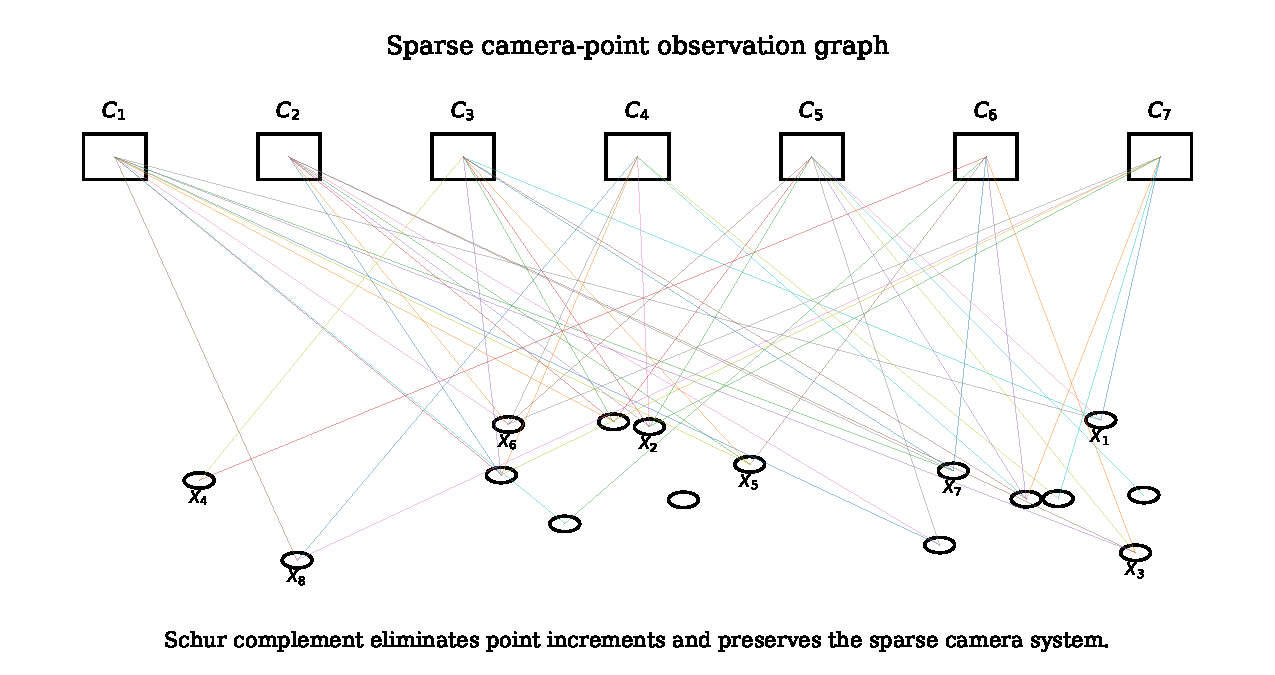
\includegraphics[width=0.86\textwidth]{bundle_adjustment_graph.pdf}
\caption{گراف دوبخشی دوربین-نقطه در تعدیل دسته‌ای. تنکی مشاهده سبب می‌شود مکمل شور و حل‌گرهای تنک بسیار مؤثر باشند.}
\label{fig:ba-graph}
\end{figure}

\subsection{آزادی پیمانه‌ای}
در بازسازی تک‌چشمی، تبدیلات تشابهی سراسری صحنه و دوربین‌ها تصویر را تغییر نمی‌دهد؛ بنابراین هفت درجه آزادی پیمانه‌ای
سه انتقال، سه چرخش و یک مقیاس وجود دارد. اگر این آزادی مهار نشود، هسین تکین می‌شود. راه‌های رایج:
ثابت‌کردن دوربین نخست، تثبیت مقیاس با فاصله معلوم یا افزودن پیشین‌های متریک.

\begin{warningbox}
گزارش تنها خطای بازفرافکنی برای \lr{SfM} کافی نیست. خطای کم می‌تواند با هندسه باریک، مقیاس نادرست، اعوجاج جذب‌شده در
ساختار یا نقاط با عمق بسیار نامطمئن همراه باشد. کیفیت باید با هندسه خط پایه، پوشش مسیر، کوواریانس و مرجع متریک ارزیابی شود.
\end{warningbox}

% =============================================================================
\section{مدل زمانی دوربین و شاتر غلتان}
% =============================================================================

در شاتر سراسری، همه سطرها در یک بازه زمانی مشترک نوردهی می‌شوند. در شاتر غلتان، زمان شروع نوردهی تابع سطر است:
\begin{equation}
t(v)=t_0+\tau v,
\label{eq:rs-time}
\end{equation}
که \(\tau\) تأخیر هر سطر است. بنابراین وضعیت نیز تابع سطر می‌شود:
\begin{equation}
\widetilde u\sim K[R(t(v))\mid t(t(v))]\widetilde X.
\label{eq:rs-camera}
\end{equation}
این رابطه ضمنی است، زیرا سطر خروجی \(v\) زمان فرافکنی را تعیین می‌کند.

\begin{figure}[H]
\centering
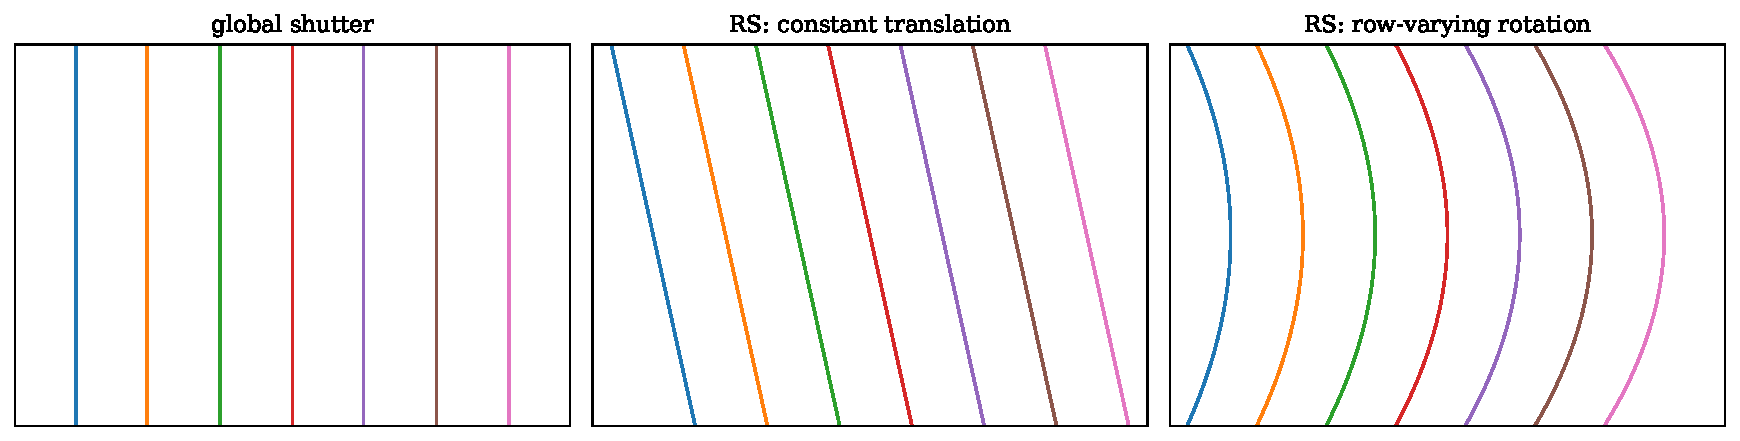
\includegraphics[width=0.88\textwidth]{rolling_shutter_geometry.pdf}
\caption{تفاوت هندسی شاتر سراسری و غلتان. در حرکت دوربین، هر سطر از وضعیت متفاوتی ثبت می‌شود و خطوط مستقیم می‌توانند کج یا خمیده شوند.}
\label{fig:rolling-shutter}
\end{figure}

برای حرکت کوتاه می‌توان وضعیت را با سرعت خطی و زاویه‌ای ثابت تقریب زد:
\begin{equation}
R(t)=\Exp((t-t_0)\skewm{\omega})R_0,
\qquad
p(t)=p_0+(t-t_0)v.
\end{equation}
اما در حرکت سریع یا غیرخطی، مدل اسپلاین زمانی و هم‌زمان‌سازی با \lr{IMU} لازم است.

\begin{futurebox}
بازسازی جدید از ویدئوی تلفن همراه باید شاتر غلتان، تاری حرکت و مسیر پیوسته دوربین را هم‌زمان مدل کند. روش‌های میدان تابشی
و گاوسی جدید، فرافکنی هر سطر یا هر نمونه نوردهی را با وضعیت متفاوت وارد رندر می‌کنند؛ این همان بازگشت مستقیم به مدل فیزیکی
دوربین درون یادگیری است.
\end{futurebox}

% =============================================================================
\section{دوربین رویدادی: هندسه بدون فریم ثابت}
% =============================================================================

دوربین رویدادی در پیکسل \(u_k\) و زمان \(t_k\) رویداد با قطبیت \(p_k\in\{-1,+1\}\) تولید می‌کند وقتی تغییر لگاریتم شدت
از آستانه \(C\) عبور کند:
\begin{equation}
\log I(u_k,t_k)-\log I(u_k,t_k-\Delta t_k)=p_kC.
\label{eq:event-model}
\end{equation}
داده خروجی مجموعه نامنظم \(e_k=(u_k,t_k,p_k)\) است، نه تصویر با نرخ فریم ثابت. هندسه پرتو همچنان برقرار است، اما
زمان هر اندازه‌گیری دقیقاً بخشی از مشاهده است.

برای جبران حرکت، رویداد به زمان مرجع با مدل حرکت و عمق وارپ می‌شود. اگر پارامتر حرکت صحیح باشد، رویدادهای متناظر با یک
لبه در تصویر انباشته‌شده تیز می‌شوند. بنابراین بیشینه‌سازی کنتراست یا واریانس تصویر رویداد، تابع هدف هندسی می‌سازد.

\begin{keybox}[تفاوت بنیادی]
در دوربین معمولی ابتدا زمان روی بازه نوردهی انتگرال گرفته و سپس تصویر تولید می‌شود؛ در دوربین رویدادی تغییرات به‌صورت
ناهمگام ثبت می‌شوند. پس مفهوم «یک وضعیت برای یک تصویر» باید جای خود را به مسیر پیوسته دوربین بدهد.
\end{keybox}

% =============================================================================
\section{دوربین تفاضل‌پذیر و بهینه‌سازی مشترک صحنه-وضعیت}
% =============================================================================

\subsection{رندر تفاضل‌پذیر}
اگر رندرگر \(\mathcal R(\theta_s,\theta_c)\) تصویر را از پارامتر صحنه \(\theta_s\) و دوربین \(\theta_c\) بسازد،
می‌توان وضعیت دوربین را از گرادیان فوتومتریک بهینه کرد:
\begin{equation}
\min_{\theta_s,\theta_c}
\sum_i\norm{I_i-\mathcal R(\theta_s,\theta_{c,i})}_1.
\label{eq:differentiable-rendering}
\end{equation}
اما این مسئله غیرمحدب و دارای ابهام صحنه-دوربین است. مقداردهی اولیه، برنامه درشت‌به‌ریز، پیشین حرکت و مدل نوردهی تعیین‌کننده‌اند.

\subsection{پرتو در میدان تابشی عصبی}
برای پیکسل \(\widetilde u\)، جهت دوربینی
\begin{equation}
d_c=\frac{K^{-1}\widetilde u}{\norm{K^{-1}\widetilde u}}
\end{equation}
و جهت جهانی \(d_w=R\trans d_c\) است. پرتو
\begin{equation}
r(s)=C+s d_w
\end{equation}
در نقاط نمونه‌برداری می‌شود. میدان تابشی چگالی \(\sigma(r(s))\) و رنگ جهت‌وابسته \(c(r(s),d_w)\) می‌دهد و رنگ پیکسل از
رندر حجمی به‌دست می‌آید:
\begin{equation}
\widehat C(r)=\int_{s_n}^{s_f}T(s)\sigma(r(s))c(r(s),d)\,ds,
\qquad
T(s)=\exp\!\left(-\int_{s_n}^{s}\sigma(r(q))dq\right).
\label{eq:nerf-render}
\end{equation}

\subsection{تنظیم دسته‌ای عصبی}
روش‌هایی مانند \lr{BARF} وضعیت‌های ناقص را همراه با میدان صحنه بهینه می‌کنند. مسئله اصلی این است که مؤلفه‌های فرکانس بالای
کدگذاری مکانی می‌توانند منظره تابع هدف نسبت به وضعیت را پرنوسان کنند؛ آموزش درشت‌به‌ریز ابتدا ساختار کم‌فرکانس را هم‌تراز
و سپس جزئیات را فعال می‌کند.

\subsection{فرافکنی گاوسی سه‌بعدی}
در \lr{3D Gaussian Splatting}، هر پرایمیتیو میانگین \(\mu\)، کوواریانس \(\Sigma\)، کد رنگ و کدری دارد. با ژاکوبین فرافکنی
\(J_\pi\)، تقریب کوواریانس دوبعدی اثر تصویر:
\begin{equation}
\Sigma_{2D}\simeq J_\pi R\Sigma R\trans J_\pi\trans
\label{eq:gaussian-projection}
\end{equation}
است. سپس بیضی‌های دوبعدی بر اساس عمق مرتب و آلفا-ترکیب می‌شوند.

\begin{figure}[H]
\centering
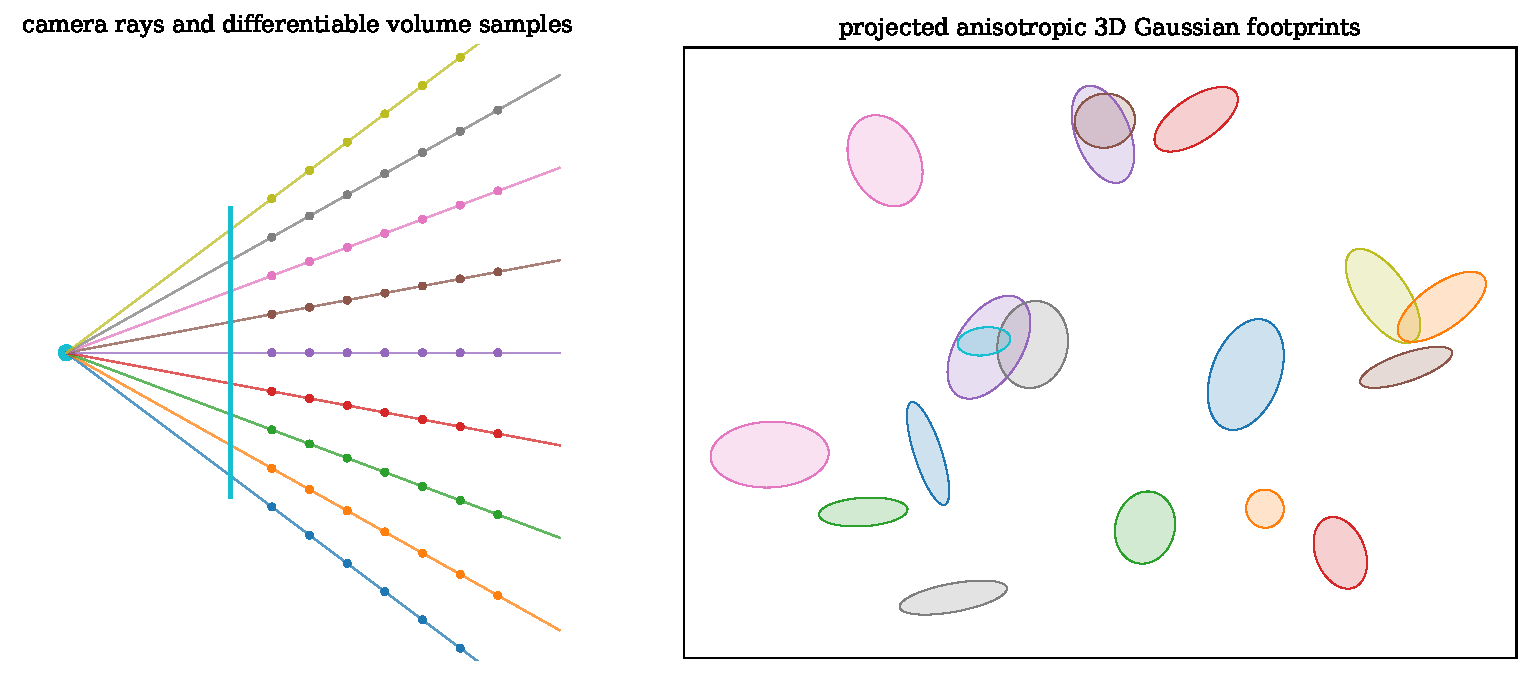
\includegraphics[width=0.9\textwidth]{differentiable_camera_rays.pdf}
\caption{چپ: نمونه‌برداری روی پرتو دوربین در رندر حجمی. راست: اثر بیضوی فرافکنی گاوسی‌های ناهمسانگرد سه‌بعدی. در هر دو، ژاکوبین دوربین جزء اصلی گرادیان است.}
\label{fig:diff-camera}
\end{figure}

\begin{warningbox}
یک بازسازی عصبی با تصویر جدید زیبا لزوماً دوربین یا هندسه متریک درست ندارد. تغییر کوچک وضعیت می‌تواند با تغییر شکل میدان
تابشی جبران شود. ارزیابی باید خطای وضعیت، عمق، سازگاری چنددیدگاهی و رفتار خارج از مسیر آموزش را نیز بسنجد.
\end{warningbox}

% =============================================================================
\section{دوربین عمومی و مدل‌های «هر دوربینی»}
% =============================================================================

روند آینده از مدل واحد سوراخ‌سوزنی به رابط عمومی پرتو حرکت می‌کند. یک مدل دوربین عمومی دو عملگر نیاز دارد:
\begin{align}
\mathcal U &: \vect u\mapsto (\vect o,\vect d), &&\text{بازفرافکنی پیکسل به پرتو},\\
\mathcal P &: \vect X\mapsto \vect u, &&\text{فرافکنی نقطه به تصویر}.
\end{align}
در دوربین مرکزی \(o=C\) برای همه پیکسل‌ها یکسان است؛ در دوربین غیرمرکزی چنین نیست.

شبکه‌های سه‌بعدی جدید نیز باید از وابستگی ضمنی به دوربین پرسپکتیو رها شوند. راه‌حل‌های هندسه-آگاه، جهت پرتو روی کره یا
نگاشت معکوس دوربین را ورودی مدل می‌کنند تا آموزش روی لنزها و میدان دیدهای متفاوت ممکن شود.

\begin{futurebox}
در دهه آینده، «ماتریس دوربین» به «مدل حسگر زمان‌مند و تفاضل‌پذیر» گسترش می‌یابد: لنز، شاتر، پاسخ تابشی، مسیر، عدم‌قطعیت
و هم‌زمانی چندحسگر همگی در یک گراف محاسباتی قرار می‌گیرند. بااین‌حال، پایه همچنان نقطه، پرتو، تبدیل صلب و قید چنددیدگاهی است.
\end{futurebox}

% =============================================================================
\section{خطا، عدم‌قطعیت و طراحی آزمایش هندسی}
% =============================================================================

\subsection{انتشار کوواریانس}
اگر \(y=f(x)\) و \(x\) کوواریانس \(\Sigma_x\) داشته باشد، تقریب مرتبه اول:
\begin{equation}
\Sigma_y\simeq J_f\Sigma_xJ_f\trans.
\label{eq:cov-propagation}
\end{equation}
برای فرافکنی، این رابطه بیضی عدم‌قطعیت پیکسلی را از عدم‌قطعیت نقطه یا وضعیت می‌سازد؛ برای مثلث‌بندی، برعکس عدم‌قطعیت
پیکسل به بیضوی سه‌بعدی تبدیل می‌شود.

\subsection{خطای پیکسل مستقل و همسان نیست}
گوشه‌های شطرنجی در تاری، اشباع یا حاشیه تصویر کوواریانس یکسان ندارند. تطابق ویژگی در امتداد لبه عدم‌قطعیت بیشتری دارد.
استفاده از وزن \(\Sigma_{ij}^{-1}\) در \eqref{eq:calib-objective} و \eqref{eq:ba} از نظر آماری درست‌تر از وزن برابر است.

\subsection{تابع هزینه مقاوم}
برای باقیمانده بزرگ، توابع هابر یا کاوشی اثر برون‌زد را محدود می‌کنند. اما هزینه مقاوم جایگزین تشخیص مدل غلط نیست؛ اگر
اعوجاج یا شاتر غلتان نادیده گرفته شود، باقیمانده «برون‌زد تصادفی» نیست و تابع مقاوم ممکن است آن را پنهان کند.

\subsection{طراحی مسیر و هدف}
اطلاعات هندسی به پوشش زاویه، عمق، میدان دید و خط پایه وابسته است. طراحی فعال نما می‌تواند دترمینان یا کوچک‌ترین مقدار ویژه
ماتریس اطلاعات را بهینه کند:
\begin{equation}
\text{D-optimal: }\max\log\det(J\trans WJ),
\qquad
\text{E-optimal: }\max\lambda_{\min}(J\trans WJ).
\end{equation}
این دیدگاه، ثبت داده را از یک کار دستی به مسئله طراحی آزمایش تبدیل می‌کند.

% =============================================================================
\section{پروتکل مهندسی کالیبراسیون و بازسازی}
% =============================================================================

\begin{enumerate}
\item \textbf{قفل‌کردن سامانه:} رزولوشن، زوم، فوکوس، پایدارسازی دیجیتال و پردازش داخلی را مشخص و ثابت کنید.
\item \textbf{انتخاب مدل:} نوع لنز و میدان دید را تعیین و ساده‌ترین مدل فیزیکی معقول را انتخاب کنید.
\item \textbf{ثبت متنوع:} هدف را در مرکز و گوشه‌ها، عمق‌ها و زاویه‌های مختلف ثبت کنید؛ از نمای تقریباً یکسان پرهیز کنید.
\item \textbf{کنترل کیفیت هدف:} اندازه خانه، تختی، چاپ و آشکارسازی زیرپیکسلی را بررسی کنید.
\item \textbf{مقداردهی اولیه:} هموگرافی/\lr{DLT} و مدل کم‌پارامتر را برای شروع به‌کار ببرید.
\item \textbf{پالایش غیرخطی:} خطای بازفرافکنی وزن‌دار و مقاوم را روی منیفلد چرخش کمینه کنید.
\item \textbf{تشخیص:} بردارهای باقیمانده را روی تصویر رسم، نماهای نامطمئن و حاشیه‌ها را جداگانه بررسی کنید.
\item \textbf{اعتبارسنجی:} بخشی از نماها یا یک شیء متریک مستقل را خارج از برازش نگه دارید.
\item \textbf{نسخه‌گذاری:} پارامترها را همراه با رزولوشن، دمای سامانه، فوکوس، زمان و شناسه دوربین ذخیره کنید.
\item \textbf{انتقال عدم‌قطعیت:} خطای کالیبراسیون را در عمق، وضعیت و تصمیم پایین‌دست منتشر کنید.
\end{enumerate}

\begin{keybox}[گزارش حداقلی قابل دفاع]
یک گزارش کالیبراسیون حرفه‌ای باید ماتریس درونی و مدل اعوجاج، تعداد و تنوع نماها، اندازه هدف، خطای هر نما، توزیع و نقشه
برداری باقیمانده، عدم‌قطعیت پارامترها، نتیجه داده اعتبارسنجی و شرایط تصویربرداری را ارائه کند. یک عدد \lr{RMS} به‌تنهایی
گزارش علمی نیست.
\end{keybox}

% =============================================================================
\section{کارگاه جامع پایتون و OpenCV}
% =============================================================================

\subsection{فرافکنی نقطه سه‌بعدی}
\begin{latin}
\begin{lstlisting}
import numpy as np

def project_points(K, R, t, X_world):
    """Project N x 3 world points to N x 2 pixels."""
    Xc = (R @ X_world.T + t.reshape(3, 1)).T
    if np.any(Xc[:, 2] <= 0):
        raise ValueError("All points must have positive camera depth")
    q = (K @ Xc.T).T
    uv = q[:, :2] / q[:, 2:3]
    return uv, Xc[:, 2]
\end{lstlisting}
\end{latin}

\subsection{خطای سامپسون برداری}
\begin{latin}
\begin{lstlisting}
def sampson_error(F, x1, x2, eps=1e-12):
    """x1 and x2 are N x 2 pixel arrays."""
    x1h = np.c_[x1, np.ones(len(x1))]
    x2h = np.c_[x2, np.ones(len(x2))]
    Fx1 = (F @ x1h.T).T
    Ftx2 = (F.T @ x2h.T).T
    numer = np.sum(x2h * Fx1, axis=1) ** 2
    denom = (Fx1[:, 0] ** 2 + Fx1[:, 1] ** 2
             + Ftx2[:, 0] ** 2 + Ftx2[:, 1] ** 2)
    return numer / np.maximum(denom, eps)
\end{lstlisting}
\end{latin}

\subsection{کالیبراسیون با کنترل خطای هر نما}
\begin{latin}
\begin{lstlisting}
rms, K, dist, rvecs, tvecs = cv2.calibrateCamera(
    object_points, image_points, image_size, None, None
)

per_view_rmse = []
for X, u, rvec, tvec in zip(object_points, image_points,
                             rvecs, tvecs):
    pred, _ = cv2.projectPoints(X, rvec, tvec, K, dist)
    residual = pred.reshape(-1, 2) - u.reshape(-1, 2)
    per_view_rmse.append(np.sqrt(np.mean(np.sum(residual**2, axis=1))))
\end{lstlisting}
\end{latin}

\begin{codecontract}
هر تابع باید قرارداد مختصات، واحد، جهت تبدیل و شکل آرایه را در \lr{docstring} اعلام کند. آزمون واحد حداقل باید شامل
مرکز تصویر، نقطه روی محور نوری، تبدیل معکوس وضعیت، تغییر اندازه تصویر و مقایسه با \texttt{cv2.projectPoints} باشد.
\end{codecontract}

\begin{workshopbox}[خروجی‌های همراه فصل]
اسکریپت \texttt{scripts/generate\_figures.py} تمام شکل‌ها و دو آزمایش عددی را تولید می‌کند:
\begin{itemize}
\item کالیبراسیون مصنوعی با پارامترهای معلوم، اعوجاج و نویز گوشه؛
\item تخمین ماتریس بنیادی و محاسبه خطای سامپسون روی دو دوربین مصنوعی.
\end{itemize}
نتایج در پوشه \texttt{outputs} ذخیره شده‌اند تا دانشجو بتواند اثر نویز و هندسه را بدون وابستگی به داده بیرونی بازتولید کند.
\end{workshopbox}

% =============================================================================
\section{آزمایش‌های پیشنهادی از پایه تا پژوهش}
% =============================================================================

\subsection{آزمایش ۱: شرطی‌بودن DLT}
مختصات نقاط را بدون نرمال‌سازی و با نرمال‌سازی حل کنید. عدد شرط \(A\)، خطای پارامتر و خطای بازفرافکنی را در نویزهای مختلف
مقایسه کنید. نشان دهید نرمال‌سازی الگوریتم را از نظر عددی تغییر می‌دهد، نه مدل هندسی را.

\subsection{آزمایش ۲: مشاهده‌پذیری کالیبراسیون}
سه رژیم داده بسازید: نماهای تقریباً روبه‌رو، نماهای متنوع، و نماهای متنوع با پوشش حاشیه. مقدار ویژه‌های \(J\trans J\)،
عدم‌قطعیت \(f_x,k_1,k_2\) و خطای اعتبارسنجی را مقایسه کنید.

\subsection{آزمایش ۳: انتخاب مدل اعوجاج}
داده را با مدل کانالا-برنت تولید و با مدل‌های ساده شعاعی، براون و کانالا-برنت برازش کنید. نمودار بردار باقیمانده و خطای
حاشیه را گزارش کنید. سپس حالت عکس را اجرا و بیش‌برازش مدل پرپارامتر را بررسی کنید.

\subsection{آزمایش ۴: تباهی دو دید}
برای خط پایه‌های مختلف، چرخش خالص، صفحه غالب و صحنه حجمی، \(F\) و \(H\) را در \lr{RANSAC} برازش کنید. نسبت درون‌زد،
خطای اعتبارسنجی و شرط مثلث‌بندی را تحلیل کنید.

\subsection{آزمایش ۵: بودجه خطای استریو}
از رابطه \eqref{eq:depth-uncertainty} یک طراحی حسگر بسازید: برای محدوده عمق و خطای مجاز، ترکیب \(f,B,\sigma_d\) را تعیین کنید.
سپس محدودیت همپوشانی و حداقل عمق را به مسئله بهینه‌سازی چندهدفه بیفزایید.

\subsection{آزمایش ۶: شاتر غلتان}
یک شبکه سه‌بعدی را با مسیر دوربین پیوسته و زمان سطر شبیه‌سازی کنید. ابتدا مدل شاتر سراسری را برازش و الگوی باقیمانده را
رسم کنید؛ سپس \(\tau\) و سرعت را وارد مدل کنید. نشان دهید تابع مقاوم به‌تنهایی خطای مدل را درمان نمی‌کند.

\subsection{آزمایش ۷: تنظیم دسته‌ای عصبی در مقیاس کوچک}
یک صحنه مصنوعی تفاضل‌پذیر با چند نقطه یا گاوسی بسازید. وضعیت‌های اولیه را اغتشاش دهید و بهینه‌سازی مشترک صحنه و دوربین را
با فعال‌سازی تدریجی فرکانس‌ها اجرا کنید. خطای وضعیت و تصویر را جداگانه گزارش کنید.

% =============================================================================
\section{تمرین‌های نظری و اثباتی}
% =============================================================================

\begin{enumerate}
\item ثابت کنید هموگرافی هشت درجه آزادی دارد و چرا مقیاس کلی قابل مشاهده نیست.
\item رابطه انتقال خط \(\ell'=H^{-\mathsf T}\ell\) را از قید برخورد استخراج کنید.
\item از مشابهت مثلث‌ها رابطه \(x=fX/Z\) را استخراج و ژاکوبین آن را نسبت به \(X,Y,Z\) محاسبه کنید.
\item نشان دهید مرکز دوربین در فضای تهی راست \(P\) قرار دارد.
\item ثابت کنید \(E=[t]_\times R\) رتبه دو دارد و \(t\) در فضای تهی چپ آن است.
\item درجه آزادی ماتریس بنیادی و اساسی را با درنظرگرفتن قیودشان به‌دست آورید.
\item خطای سامپسون را با خطی‌سازی قید اپی‌پولار نسبت به تصحیح چهار مختصات استخراج کنید.
\item برای استریو تصحیح‌شده، رابطه \(Z=fB/d\) و کوواریانس آن را با نویز هم‌بسته در دو تصویر استخراج کنید.
\item قیدهای ژانگ \eqref{eq:zhang-constraints} را از تعامد ستون‌های چرخش اثبات کنید.
\item نشان دهید در بازسازی تک‌چشمی، تبدیل تشابهی سراسری تصاویر را ثابت می‌گذارد.
\item ساختار مکمل شور \eqref{eq:schur} را از حذف بلوکی \(\delta_p\) استخراج کنید.
\item برای یک دوربین شاتر غلتان با ترجمه افقی ثابت، شکل خط عمودی تصویرشده را به‌صورت تابع سطر به‌دست آورید.
\item کوواریانس دوبعدی گاوسی فرافکنی‌شده \eqref{eq:gaussian-projection} را از تقریب مرتبه اول به‌دست آورید.
\item نشان دهید چرا مدل پرسپکتیو در \(\theta\to90^\circ\) واگرا می‌شود ولی مدل هم‌فاصله محدود می‌ماند.
\item یک مثال بسازید که خطای بازفرافکنی کم، اما عمق سه‌بعدی بسیار نامطمئن باشد.
\end{enumerate}

% =============================================================================
\section{پروژه‌های پایان فصل}
% =============================================================================

\subsection{پروژه A: سامانه ممیزی کالیبراسیون}
ابزاری بنویسید که علاوه بر اجرای کالیبراسیون، پوشش تصویر، تنوع وضعیت، باقیمانده برداری، خطای هر نما، حساسیت حذف-یک-نما،
کوواریانس تقریبی و اعتبارسنجی نگه‌داشته‌شده را گزارش کند. خروجی باید یک گزارش \lr{HTML/PDF} و فایل پارامتر نسخه‌گذاری‌شده باشد.

\subsection{پروژه B: کتابخانه دوربین عمومی}
یک رابط نرم‌افزاری برای \texttt{project} و \texttt{unproject} بسازید و مدل‌های پرسپکتیو، براون، کانالا-برنت و همه‌جهته را
پیاده کنید. آزمون رفت‌وبرگشت، ژاکوبین تحلیلی/خودکار و رفتار حاشیه میدان دید را مقایسه کنید.

\subsection{پروژه C: بازسازی با مدل شاتر غلتان}
ویدئوی تلفن همراه را با نرخ سطر معلوم یا تخمینی بازسازی کنید. خط لوله شاتر سراسری و غلتان را از نظر خطای وضعیت، خمیدگی خطوط،
کیفیت نقاط سه‌بعدی و هزینه محاسباتی مقایسه کنید.

\subsection{پروژه D: تنظیم مشترک دوربین و میدان صحنه}
یک بازنمایی کوچک \lr{NeRF} یا گاوسی را روی صحنه مصنوعی آموزش دهید، سپس وضعیت‌های ورودی را اغتشاش دهید. اثر مقداردهی اولیه،
کدگذاری فرکانسی، پیشین مسیر و مدل اعوجاج را روی همگرایی وضعیت مطالعه کنید.

% =============================================================================
\section{پرامپت پیشنهادی برای Codex}
% =============================================================================

\begin{latin}
\begin{lstlisting}[language={}]
Act as a senior computer-vision geometry engineer. Build a reproducible
Python project for Chapter 6, "Image and Camera Geometry".

Requirements:
1. Implement explicit coordinate conventions and unit-tested SE(3),
   pinhole projection, Brown-Conrady distortion, Kannala-Brandt fisheye,
   homography DLT, normalized eight-point F estimation, Sampson error,
   linear/nonlinear triangulation, and stereo depth uncertainty.
2. Generate synthetic calibration observations with known intrinsics,
   distortion, board geometry, and camera poses. Estimate parameters with
   OpenCV and independently verify projection and residuals.
3. Diagnose calibration using per-view RMSE, vector residual maps,
   held-out views, leave-one-view-out sensitivity, Jacobian singular values,
   and approximate covariance.
4. Simulate degenerate configurations: fronto-parallel calibration views,
   pure rotation, planar scenes, short stereo baseline, and rolling shutter.
5. Add robust two-view estimation with RANSAC and compare algebraic,
   point-to-line, and Sampson residuals.
6. Create a small differentiable camera experiment in PyTorch that jointly
   optimizes camera pose and 3D points or Gaussian primitives. Report both
   photometric loss and metric pose/structure error.
7. Save every figure as PDF and PNG, every metric as CSV/JSON, and create a
   Persian README with exact commands for Windows and Linux.
8. Do not silently switch coordinate systems. Every function must state
   world-to-camera versus camera-to-world, pixel ordering, axis directions,
   and units. Add tests against cv2.projectPoints.
9. Use fixed random seeds, type hints, validation, and informative errors.
10. Never fabricate numerical results; run all experiments and insert the
    actual outputs into the report.
\end{lstlisting}
\end{latin}

% =============================================================================
\section{تقسیم پیشنهادی ویدئوهای ۱۵ دقیقه‌ای}
% =============================================================================

\begin{videobox}
\begin{longtable}{p{1.2cm}p{5.1cm}p{8.2cm}}
\toprule
بخش & عنوان & هدف و خروجی\\
\midrule
۱ & پیکسل به‌مثابه پرتو & ابهام عمق و زنجیره مدل دوربین\\
۲ & مختصات همگن & نقطه، خط، برخورد و نقطه بی‌نهایت\\
۳ & هموگرافی & گروه تصویری و سلسله‌مراتب تبدیلات\\
۴ & چرخش سه‌بعدی & \(SO(3)\)، رودریگز و نمایش‌ها\\
۵ & وضعیت دوربین & \(SE(3)\)، مرکز دوربین و قراردادها\\
۶ & سوراخ‌سوزنی & استخراج \(x=fX/Z\) و ماتریس دوربین\\
۷ & پارامترهای درونی & فاصله کانونی، نقطه اصلی، رزولوشن و میدان دید\\
۸ & ژاکوبین فرافکنی & مشتق نسبت به نقطه و وضعیت\\
۹ & لنز نازک & فوکوس، عمق میدان و تاری عمق‌وابسته\\
۱۰ & اعوجاج براون & شعاعی، مماسی و خطاهای مدل\\
۱۱ & چشم‌ماهی & قوانین فرافکنی و مدل کانالا-برنت\\
۱۲ & دوربین همه‌جهته & مدل مرکزی و رابط پرتو عمومی\\
۱۳ & هندسه تک‌دید & نقاط گریز، خط افق و منهتن\\
۱۴ & هموگرافی صفحه & استخراج، تصحیح و اندازه‌گیری\\
۱۵ & DLT & ساخت دستگاه و نرمال‌سازی\\
۱۶ & روش ژانگ & قیود \(B=K^{-T}K^{-1}\)\\
۱۷ & پالایش کالیبراسیون & خطای بازفرافکنی، LM و تابع مقاوم\\
۱۸ & ممیزی کالیبراسیون & باقیمانده، کوواریانس و طراحی نما\\
۱۹ & هندسه اپی‌پولار & \(E\)، \(F\)، اپی‌پل و خط اپی‌پولار\\
۲۰ & هشت‌نقطه‌ای & نرمال‌سازی، قید رتبه و سامپسون\\
۲۱ & RANSAC و تباهی & صفحه غالب، چرخش خالص و خط پایه کم\\
۲۲ & وضعیت نسبی & تجزیه \(E\)، مثبت‌بودن عمق و مقیاس\\
۲۳ & مثلث‌بندی & حل خطی، حل هندسی و عدم‌قطعیت\\
۲۴ & استریو & تصحیح، اختلاف منظر و طراحی خط پایه\\
۲۵ & PnP & وضعیت مطلق و حل‌گرهای مینیمال\\
۲۶ & SfM & خط لوله بازسازی چنددیدگاهی\\
۲۷ & تعدیل دسته‌ای & تنکی، مکمل شور و آزادی پیمانه‌ای\\
۲۸ & شاتر غلتان & مدل زمان سطر و هندسه متحرک\\
۲۹ & دوربین رویدادی & مدل کنتراست و وارپ زمانی\\
۳۰ & دوربین تفاضل‌پذیر & رندر و بهینه‌سازی وضعیت\\
۳۱ & NeRF و BARF & پرتو، رندر حجمی و تنظیم عصبی\\
۳۲ & Gaussian Splatting & فرافکنی کوواریانس و رندر سریع\\
۳۳ & آزمایش کالیبراسیون & اجرای کد و تحلیل CSV\\
۳۴ & پروژه پژوهشی & طراحی یک سامانه ممیزی و مدل هر دوربینی\\
\bottomrule
\end{longtable}
\end{videobox}

% =============================================================================
\section{جمع‌بندی و پل به فصل هفتم}
% =============================================================================

\begin{summarybox}
\begin{enumerate}
\item هر پیکسل در مدل مرکزی یک پرتو است؛ عمق تک‌دید ذاتاً مبهم است.
\item مختصات همگن انتقال، پرسپکتیو، نقاط بی‌نهایت و برخورد را در زبان ماتریسی واحد قرار می‌دهد.
\item ماتریس دوربین \(P=K[R|t]\) ترکیب وضعیت و پارامتر درونی است؛ قرارداد جهت تبدیل باید صریح باشد.
\item چرخش روی منیفلد \(SO(3)\) و وضعیت روی \(SE(3)\) قرار دارد؛ اغتشاش لی ابزار طبیعی بهینه‌سازی هندسی است.
\item اعوجاج دوربین واقعی تنها با یک ضریب شعاعی خلاصه نمی‌شود؛ مدل باید با نوع لنز و داده اعتبارسنجی انتخاب شود.
\item روش ژانگ از هموگرافی صفحه و تعامد ستون‌های چرخش، درونی‌ها را مقداردهی اولیه و سپس همه پارامترها را غیرخطی پالایش می‌کند.
\item خطای بازفرافکنی کم شرط لازم است، نه کافی؛ پوشش، باقیمانده، عدم‌قطعیت و اعتبارسنجی مستقل ضروری‌اند.
\item هندسه دو دید با قید \(x_2^TFx_1=0\) جست‌وجوی تطابق را محدود و وضعیت نسبی را تا مقیاس بازیابی می‌کند.
\item دقت عمق استریو با مربع فاصله افت می‌کند؛ خط پایه و هندسه ثبت بخشی از طراحی برآوردگرند.
\item تعدیل دسته‌ای بازسازی و دوربین را مشترکاً بهینه می‌کند و تنکی گراف مشاهده با مکمل شور بهره‌برداری می‌شود.
\item شاتر غلتان و دوربین رویدادی نشان می‌دهند که زمان باید جزء مدل هندسی مشاهده باشد.
\item NeRF، BARF و Gaussian Splatting هندسه دوربین را حذف نکرده‌اند؛ آن را به یک گراف تفاضل‌پذیر درون بهینه‌سازی صحنه برده‌اند.
\item فصل هفتم می‌تواند بر استخراج لبه، ویژگی و تطابق بنا شود؛ زیرا اکنون می‌دانیم ویژگی در کدام هندسه و با کدام عدم‌قطعیت اندازه‌گیری می‌شود.
\end{enumerate}
\end{summarybox}

\backmatter
\chapter*{منابع منتخب فصل}
\addcontentsline{toc}{chapter}{منابع منتخب فصل}

\begin{latin}
\begin{thebibliography}{99}

\bibitem{hartley2004}
R. Hartley and A. Zisserman,
\textit{Multiple View Geometry in Computer Vision}, 2nd ed., Cambridge University Press, 2004.

\bibitem{szeliski2022}
R. Szeliski,
\textit{Computer Vision: Algorithms and Applications}, 2nd ed., Springer, 2022.

\bibitem{ma2004}
Y. Ma, S. Soatto, J. Kosecka, and S. Sastry,
\textit{An Invitation to 3-D Vision}, Springer, 2004.

\bibitem{faugeras1993}
O. Faugeras,
\textit{Three-Dimensional Computer Vision: A Geometric Viewpoint}, MIT Press, 1993.

\bibitem{hartley1997eight}
R. I. Hartley,
``In defense of the eight-point algorithm,''
\textit{IEEE Transactions on Pattern Analysis and Machine Intelligence}, vol. 19, no. 6, pp. 580--593, 1997.

\bibitem{nister2004five}
D. Nistér,
``An efficient solution to the five-point relative pose problem,''
\textit{IEEE Transactions on Pattern Analysis and Machine Intelligence}, vol. 26, no. 6, pp. 756--770, 2004.

\bibitem{fischler1981ransac}
M. A. Fischler and R. C. Bolles,
``Random sample consensus: A paradigm for model fitting with applications to image analysis and automated cartography,''
\textit{Communications of the ACM}, vol. 24, no. 6, pp. 381--395, 1981.

\bibitem{zhang2000}
Z. Zhang,
``A flexible new technique for camera calibration,''
\textit{IEEE Transactions on Pattern Analysis and Machine Intelligence}, vol. 22, no. 11, pp. 1330--1334, 2000.

\bibitem{brown1966}
D. C. Brown,
``Decentering distortion of lenses,''
\textit{Photogrammetric Engineering}, vol. 32, no. 3, pp. 444--462, 1966.

\bibitem{kannala2006}
J. Kannala and S. S. Brandt,
``A generic camera model and calibration method for conventional, wide-angle, and fish-eye lenses,''
\textit{IEEE Transactions on Pattern Analysis and Machine Intelligence}, vol. 28, no. 8, pp. 1335--1340, 2006.

\bibitem{mei2007}
C. Mei and P. Rives,
``Single view point omnidirectional camera calibration from planar grids,''
in \textit{Proceedings of ICRA}, pp. 3945--3950, 2007.

\bibitem{triggs2000}
B. Triggs, P. McLauchlan, R. Hartley, and A. Fitzgibbon,
``Bundle adjustment -- a modern synthesis,''
in \textit{Vision Algorithms: Theory and Practice}, pp. 298--372, Springer, 2000.

\bibitem{agarwal2010}
S. Agarwal, N. Snavely, S. M. Seitz, and R. Szeliski,
``Bundle adjustment in the large,''
in \textit{Proceedings of ECCV}, pp. 29--42, 2010.

\bibitem{schoenberger2016sfm}
J. L. Schönberger and J.-M. Frahm,
``Structure-from-motion revisited,''
in \textit{Proceedings of CVPR}, pp. 4104--4113, 2016.

\bibitem{schoenberger2016mvs}
J. L. Schönberger, E. Zheng, M. Pollefeys, and J.-M. Frahm,
``Pixelwise view selection for unstructured multi-view stereo,''
in \textit{Proceedings of ECCV}, pp. 501--518, 2016.

\bibitem{meingast2005}
M. Meingast, C. Geyer, and S. Sastry,
``Geometric models of rolling-shutter cameras,''
arXiv:cs/0503076, 2005.

\bibitem{oth2013}
L. Oth, P. Furgale, L. Kneip, and R. Siegwart,
``Rolling shutter camera calibration,''
in \textit{Proceedings of CVPR}, pp. 1360--1367, 2013.

\bibitem{dai2016rs}
Y. Dai, H. Li, and L. Kneip,
``Rolling shutter camera relative pose: Generalized epipolar geometry,''
in \textit{Proceedings of CVPR}, pp. 4132--4140, 2016.

\bibitem{gallego2020event}
G. Gallego et al.,
``Event-based vision: A survey,''
\textit{IEEE Transactions on Pattern Analysis and Machine Intelligence}, vol. 44, no. 1, pp. 154--180, 2022.

\bibitem{mildenhall2020nerf}
B. Mildenhall et al.,
``NeRF: Representing scenes as neural radiance fields for view synthesis,''
in \textit{Proceedings of ECCV}, pp. 405--421, 2020.

\bibitem{lin2021barf}
C.-H. Lin, W.-C. Ma, A. Torralba, and S. Lucey,
``BARF: Bundle-adjusting neural radiance fields,''
in \textit{Proceedings of ICCV}, pp. 5741--5751, 2021.

\bibitem{kerbl2023gs}
B. Kerbl, G. Kopanas, T. Leimkühler, and G. Drettakis,
``3D Gaussian splatting for real-time radiance field rendering,''
\textit{ACM Transactions on Graphics}, vol. 42, no. 4, 2023.

\bibitem{niu2024rsnerf}
M. Niu, T. Chen, Y. Zhan, Z. Li, X. Ji, and Y. Zheng,
``RS-NeRF: Neural radiance fields from rolling shutter images,''
arXiv:2407.10267, 2024.

\bibitem{hahn2025rs}
M. A. Hahn et al.,
``Order-one rolling shutter cameras,''
in \textit{Proceedings of CVPR}, 2025.

\bibitem{opencvcalib}
OpenCV Development Team,
``Camera Calibration and 3D Reconstruction -- calib3d module,''
OpenCV documentation, accessed 2026.

\bibitem{colmap}
J. L. Schönberger et al.,
``COLMAP: General-purpose structure-from-motion and multi-view stereo,''
software and documentation, accessed 2026.

\bibitem{ceres}
S. Agarwal, K. Mierle, and The Ceres Solver Team,
``Ceres Solver,'' software and bundle-adjustment tutorials, accessed 2026.

\bibitem{pytorch3d}
N. Ravi et al.,
``Accelerating 3D deep learning with PyTorch3D,''
arXiv:2007.08501, 2020.

\end{thebibliography}
\end{latin}

\chapter*{راهنمای کامپایل، فونت و اجرای آزمایش‌ها}
\addcontentsline{toc}{chapter}{راهنمای کامپایل، فونت و اجرای آزمایش‌ها}

فایل با \lr{XeLaTeX} کامپایل می‌شود. در \lr{TeXstudio}، کامپایلر پیش‌فرض را روی \lr{XeLaTeX} قرار دهید و برای تکمیل
فهرست مطالب دو بار اجرا کنید. فونت اصلی \lr{Amiri}، فونت لاتین \lr{DejaVu Serif} و فونت کد
\lr{DejaVu Sans Mono} است؛ برای هر سه جایگزین خودکار تعریف شده است و هیچ فایل فونتی در بسته قرار نگرفته است.

برای تولید شکل‌ها و خروجی‌ها:
\begin{latin}
\begin{lstlisting}[language=bash]
python -m venv .venv
# Windows: .venv\Scripts\activate
# Linux/macOS: source .venv/bin/activate
pip install -r requirements.txt
python scripts/generate_figures.py
xelatex image_processing_next_decade_ch06_fa.tex
xelatex image_processing_next_decade_ch06_fa.tex
\end{lstlisting}
\end{latin}

\end{document}
